%% thesis.tex 2014/04/11
%
% Based on sample files of unknown authorship.
%
% The Current Maintainer of this work is Paul Vojta.

\documentclass[masters]{ucbthesis}
\usepackage{biblatex}
\addbibresource{references.bib}
\usepackage{float}
\usepackage{rotating} % provides sidewaystable and sidewaysfigure
\usepackage[outputdir=build]{minted}
\usepackage{amsmath}
\usepackage{siunitx}
\usepackage{caption}
\usepackage[american,siunitx,emptypmoscircle]{circuitikz}
\usepackage{subcaption}
\usemintedstyle{xcode}
\setminted{fontsize=\small}

% hyperref should be imported last.
\usepackage{hyperref}

% To compile this file, run "latex thesis", then "biber thesis"
% (or "bibtex thesis", if the output from latex asks for that instead),
% and then "latex thesis" (without the quotes in each case).

% Double spacing, if you want it.  Do not use for the final copy.
% \def\dsp{\def\baselinestretch{2.0}\large\normalsize}
% \dsp

% If the Grad. Division insists that the first paragraph of a section
% be indented (like the others), then include this line:
% \usepackage{indentfirst}

\addtolength{\abovecaptionskip}{\baselineskip}

\newtheorem{theorem}{Jibberish}


\hyphenation{mar-gin-al-ia}
\hyphenation{bra-va-do}

\begin{document}

% Declarations for Front Matter

\title{A Composable Mixed-Signal Generator Framework with Applications to an SRAM Compiler}
\author{Rahul Kumar}
\degreesemester{Spring}
\degreeyear{2023}
\degree{Master of Science}
\chair{Professor Borivoje Nikoli\'{c}}
\othermembers{Professor Vladimir Stojanovi\'{c}}
% For a co-chair who is subordinate to the \chair listed above
% \cochair{Professor Benedict Francis Pope}
% For two co-chairs of equal standing (do not use \chair with this one)
% \cochairs{Professor Richard Francis Sony}{Professor Benedict Francis Pope}
\numberofmembers{2}
% Previous degrees are no longer to be listed on the title page.
% \prevdegrees{B.A. (University of Northern South Dakota at Hoople) 1978 \\
%   M.S. (Ed's School of Quantum Mechanics and Muffler Repair) 1989}
\field{Electrical Engineering and Computer Sciences}
% Designated Emphasis -- this is optional, and rare
% \emphasis{Colloidal Telemetry}
% This is optional, and rare
% \jointinstitution{University of Western Maryland}
% This is optional (default is Berkeley)
% \campus{Berkeley}

% For a masters thesis, replace the above \documentclass line with
% \documentclass[masters]{ucbthesis}
% This affects the title and approval pages, which by default calls this
% document a "dissertation", not a "thesis".

\maketitle
% Delete (or comment out) the \approvalpage line for the final version.
\approvalpage
\copyrightpage

% (This file is included by thesis.tex; you do not latex it by itself.)

\begin{abstract}

% The text of the abstract goes here.  If you need to use a \section
% command you will need to use \section*, \subsection*, etc. so that
% you don't get any numbering.  You probably won't be using any of
% these commands in the abstract anyway.

Invasive brag; forbearance.

\end{abstract}



\begin{frontmatter}

% You can delete the \clearpage lines if you don't want these to start on
% separate pages.

\tableofcontents
\clearpage
\listoffigures
\clearpage
\listoftables

\begin{acknowledgements}

I would first like to thank my brother Rohan for his significant contributions
to much of the work presented in this thesis. I would also like to thank
my advisor, Professor Borivoje Nikoli\'{c}, for his advice and unwavering support.
I would like to further thank Dan Fritchman, Arya Reais-Parsi, and Aviral Pandey
for their ideas and discussion on automation for circuit design, as well as for
writing some of the software libraries from which Substrate draws inspiration.
I would like to thank Felicia Guo, for designing the StrongARM latches used in SRAM22;
Harrison Liew, for helping set up tools for integrating SRAM22 into digital flows; and
Nayiri Krzysztofowicz, for exercising these digital flows.
I would like to thank Brian Richards, for his help over the years in resolving
issues with infrastructure and permissions.

\end{acknowledgements}

\end{frontmatter}

\pagestyle{headings}

% (Optional) \part{First Part}

\chapter{Introduction}

\section{Motivation}

Chip design is expensive, with NRE costs in the ballpark of millions to
hundreds of millions of dollars per chip \cite{horowitz}.
With ever-changing process nodes, porting IP blocks and tool configurations
across processes becomes a painstaking endeavor.
While digital circuits can be produced mostly automatically from RTL,
no such procedure for analog circuits is in widespread use.
The result is that analog blocks are, by and large, designed by hand,
laid out by hand, and verified by hand, with limited reuse of methodology.
Furthermore, only a small portion of analog design time is spent designing
truly custom blocks. The majority is spent designing and integrating
mostly standard blocks, such as ADCs, PLLs, and LDOs.

Generators have emerged as a solution to the problem of encoding design
methodology and enabling greater automation and reuse \cite{align, template-driven-analog}.
Generator frameworks allow users to write code that accepts some set of parameters
and produces instances of a circuit. While writing a programmatic generator
may sound good in principle, there are almost always times when it is simply
faster to design or lay out a circuit by hand. This is especially the case
when designing circuits that exploit process-specific devices or design rules.
Thus, a good generator framework must make it easy to incorporate designs
produced outside the framework.

The Berkeley Analog Generator (BAG) is one generator framework developed
at UC Berkeley \cite{bag}. Although BAG has been used to design a variety
of circuits \cite{serdes-gen}, it has some limitations.
BAG is closely intertwined with Cadence Virtuoso, and although there
are ongoing efforts to remove this dependency, BAG generators still require
Virtuoso, at least for initial setup. For open-source processes such as the
Skywater 130nm process, the requirement to have access to Virtuoso
makes it difficult to write a standalone generator.
Additionally, BAG provides relatively few primitives for generating
area-constrained layouts. The default transistor cells provided by BAG
PDK plugins are difficult to customize, since BAG expects them to have
certain properties (eg. particular gate/source/drain pitches). Fitting
the existing BAG template cells into pitch-constrained layout environments
is not always possible.
Another limitation is in routing flexibility. BAG routes are usually specified
by assigning nets to track indexes via a YAML file. BAG does not support
automatic signal routing.
Finally, the use of Python as a language for writing generators precludes strict type-checking,
leading to runtime errors that could easily have been prevented at compile time.
Python also suffers from low performance, meaning that performance-sensitive algorithms
must be written in another language and then wrapped in a Python API. This makes
writing flexible layout algorithms much more tedious.

As a result, we believe that there is room for significant improvements in
analog generator workflows. 

\section{Thesis Organization}

Chapter \ref{sec:substrate} provides a high-level overview of Substrate, a framework
for writing analog/mixed-signal generators.
Chapter \ref{sec:sram22} describes SRAM22, an open-source configurable SRAM generator
build on Substrate. Chapter \ref{sec:conclusion} provides a conclusion and suggests
future directions of work.

\chapter{Substrate}

\section{Architecture}
\subsection{Guiding Principles}

Substrate aims to adhere to a few guiding principles:
\begin{enumerate}
\item Performance is flexibility. This holds true for both software and hardware.
\item Good APIs allow you to be lazy.
\item Methodology as a library. Substrate aims to be unopinionated about how you design and lay out your circuits.
  Frameworks that more rigidly prescribes how circuits are designed (eg. a library for strictly gridded layout)
  can be written as libraries using the lower-level primitives in Substrate.
  Substrate PDK plugins, for example, are simply libraries that implement a set of required functions.
  Substrate itself is a library, which means that it can be used in any Rust project or library by simply adding it to a Rust project's dependency list. Consequently, there is no such thing as a "Substrate workspace."
\end{enumerate}

\subsection{Contexts}

Substrate holds all state in a data structure called a \textbf{context}.
The context caches circuits that have been generated, and stores a handle to plugins (eg. for simulation or LVS) that have been initialized.
The context is thread safe and internally synchronized, so users can run multiple Substrate generators in parallel.

\subsection{Components}

The primary building block in Substrate is a \textbf{component}.
Substrate components are analogous to "cells" or "modules" in other design systems.
Components accept a set of parameters, and produce zero or more \textbf{views}.
Substrate currently supports schematic, layout, and timing views,
though other views will likely be added in the future.

In the Rust language, a type is considered a component if it implements the \verb|Component| trait shown below:

\begin{minted}{rust}
pub trait Component: Any {
    type Params: Serialize;
    fn new(params: &Self::Params, ctx: &SubstrateCtx) -> Result<Self>
    where
        Self: Sized;
    fn name(&self) -> ArcStr {
        // ...
    }
    fn schematic(&self, ctx: &mut SchematicCtx) -> Result<()> {
        // ...
    }
    fn layout(&self, ctx: &mut LayoutCtx) -> Result<()> {
        // ...
    }
}
\end{minted}

Components can contain instances of other components.

Substrate can perform the following operations on components:
\begin{itemize}
\item Export a schematic to a SPICE netlist
\item Export a layout to GDS.
\item Run LVS, DRC, or PEX, if an appropriate tool plugin is installed.
\end{itemize}

\subsection{Testbenches}
All testbenches are components with schematic views. This schematic view should be used to instantiate voltage sources and the block being simulated.

Testbenches must also implement the \verb|Testbench| trait, which provides hooks for:
\begin{itemize}
\item Setting up simulator analyses
\item Including external libraries, if necessary
\item Processing simulator output data
\end{itemize}

Substrate testbenches are expected to provide the name of their ground net.
Prior to simulation, Substrate will connect this net to the global ground net of the simulator (typically node \verb|0|).

\subsection{Process Development Kits} \label{sec:pdks}

Process development kits (PDKs) are ordinary Rust libraries that provide a type implementing the \verb|Pdk| trait shown below:

\begin{minted}{rust}
pub trait Pdk {
    fn name(&self) -> &'static str;
    fn process(&self) -> &'static str;
    fn lengths(&self) -> Units;
    fn voltages(&self) -> SiPrefix;
    fn layers(&self) -> Layers;
    fn supplies(&self) -> Supplies;
    /// Retrieves the list of MOSFETs available in this PDK.
    fn mos_devices(&self) -> Vec<MosSpec>;
    /// Provide the SPICE netlist for a MOSFET with the given parameters.
    ///
    /// The drain, gate, source, and body ports are named
    /// \verb|d|, \verb|g|, \verb|s|, and \verb|b|, respectively.
    fn mos_schematic(&self, ctx: &mut SchematicCtx, params: &MosParams) -> Result<()>;
    /// Draws MOSFETs with the given parameters
    fn mos_layout(&self, ctx: &mut LayoutCtx, params: &LayoutMosParams) -> Result<()>;
    /// Draws a via with the given params in the given context.
    fn via_layout(&self, ctx: &mut LayoutCtx, params: &ViaParams) -> Result<()>;
    /// The grid on which all layout geometry must lie.
    fn layout_grid(&self) -> i64;
    /// Called before running simulations.
    ///
    /// Allows the PDK to include model libraries, configure simulation
    /// options, and/or write relevant files.
    fn pre_sim(&self, _ctx: &mut PreSimCtx) -> Result<()> {
        Ok(())
    }
    /// Returns data that should be prepended to generated netlists,
    /// depending on the netlist purpose and the process corner.
    fn includes(&self, purpose: NetlistPurpose) -> Result<IncludeBundle> {
        Ok(Default::default())
    }
    /// Returns a database of the standard cell libraries available in the PDK.
    fn standard_cells(&self) -> Result<StdCellDb> {
        Ok(StdCellDb::new())
    }
    /// Returns a database of the available process corners.
    fn corners(&self) -> Result<CornerDb> {
        Ok(CornerDb::new())
    }
}
\end{minted}

The \verb|layers| function returns a layer database, which includes information on GDS layer numbers, layer purposes, and additional metadata (eg. identifying which metal/via layers and providing layer names).
The \verb|standard_cells| provides zero or more standard cell libraries. The standard cell API is described further in TODO.
The \verb|corners| function provides zero or more process corners. Depending on the corner the user selects, the PDK can include a different set of model libraries.
The \verb|mos_schematic| and \verb|mos_layout| functions instantiate PDK-specific CMOS devices in schematic and layout mode, respectively.
For further information on the other functions available, see the Substrate documentation.

Since PDKs are simply libraries, they are free to provide functions other than the ones specified here.
For instance, a PDK may export a component for a unit capacitor, even though Substrate currently does not
have a unified API for creating capacitors.

\section{Schematic Entry}

A very simple schematic generator, which produces an ideal resistive voltage divider, is shown below:

\begin{minted}{rust}
impl Component for VDivider {
    // ...
    
  fn schematic(&self, ctx: &mut SchematicCtx) -> Result<()> {
      let out = ctx.port("out", Direction::Output);
      let vdd = ctx.port("vdd", Direction::InOut);
      let vss = ctx.port("vss", Direction::InOut);

      ctx.instantiate::<Resistor>(&SiValue::new(2, SiPrefix::Kilo))?
          .with_connections([("p", vdd), ("n", out)])
          .named("R1")
          .add_to(ctx);

      ctx.instantiate::<Resistor>(&SiValue::new(1, SiPrefix::Kilo))?
          .with_connections([("p", out), ("n", vss)])
          .named("R2")
          .add_to(ctx);
      Ok(())
  }
}
\end{minted}

This starts by declaring three ports: \verb|out|, \verb|vdd|, and \verb|vss|, with the specified directions.
We then instantiate 2 resistors: one with value $\SI{2}{\kilo\ohm}$, and one with value $\SI{1}{\kilo\ohm}$,
and connect them appropriately.

This schematic can easily be exported to a SPICE netlist:

\begin{minted}{rust}
ctx.write_schematic_to_file::<VDivider>(&NoParams, path);
\end{minted}

Netlist generation in Substrate involves several passes:
+ Netlists are preprocessed to resolve duplicate net, instance, or module names.
+ The netlist is validated for correctness. This currently involves 3 analyses:
  - A name-validity analysis checks for duplicate or SPICE-incompatible names.
  - A netlist connectivity analysis verifies that all modules have their ports connected and that all widths are matched.
  - A net driver analysis verifies that all input ports are driven by at least one source and produces warnings if nets have multiple drivers.
+ A netlisting plugin maps the in-memory representation of Substrate components to simulator specific syntax and writes the content of the netlist to an output stream (usually a file).


\section{Layout Entry} \label{sec:layout-entry}

Most analog generators, Substrate included, produce layouts in roughly three steps:
+ Generate or import sub-components.
+ Place sub-components.
+ Route between sub-components.

The first step is described in more detail in \ref{sec:subcomponent-layout-generation},
the second step in \ref{sec:placement-utilities}, and the third in \ref{sec:routing}.

\subsection{Subcomponent Layout Generation} \label{sec:subcomponent-layout-generation}

This section describes how base-layer components, such as transistors, resistors, and capacitors, can be generated or imported into Substrate.

\subsubsection{Hard Macros} \label{sec:hard-macros}
Hard macros allow users to import arbitrary layouts into Substrate, and use them as if they were regular components. They are useful when you are incorporating externally-provided cells (eg. provided by a foundry or generated by a tool other than Substrate), or where writing generator code would be slower and have little benefit over a hand-drawn layout.

Hard macros can be incorporated into Substrate using the \verb|hard_macro| attribute, which is a Rust procedural macro.

\begin{minted}{rust}
#[hard_macro(
    name = "sram_sp_cell",
    pdk = "sky130-open",
    path_fn = "path",
    gds_cell_name = "sky130_fd_bd_sram__sram_sp_cell_opt1",
    spice_subckt_name = "sram_sp_cell"
)]
pub struct SpCell;
\end{minted}

The arguments to the procedural macro allow the user to specify a path function. The path function accepts a single argument – a view type (ie. schematic or layout) – and returns the path at which the appropriate view is stored (ie. a SPICE netlist or a GDS file, respectively).

Hard macros can then be instantiated as regular Substrate components, in both layout and schematic mode:
\begin{minted}{rust}
ctx.instantiate::<SpCell>(&NoParams);
\end{minted}

\subsubsection{Raw Layout Utilities}

In the spirit of giving the user complete control over generated layout, Substrate allows users to
specify layouts down to individual polygons. To create layout geometry, users specify a layer
(obtained from the PDK API described in \ref{sec:pdks}) and a shape.

There is a rich system of utilities for manipulating rectangular geometry, since rectangles are the
predominant shape in integrated circuit layouts. The Substrate documentation lists the full set of
helpers; an image of one page of the documentation is included here for reference.

\begin{figure}[htb] \centering
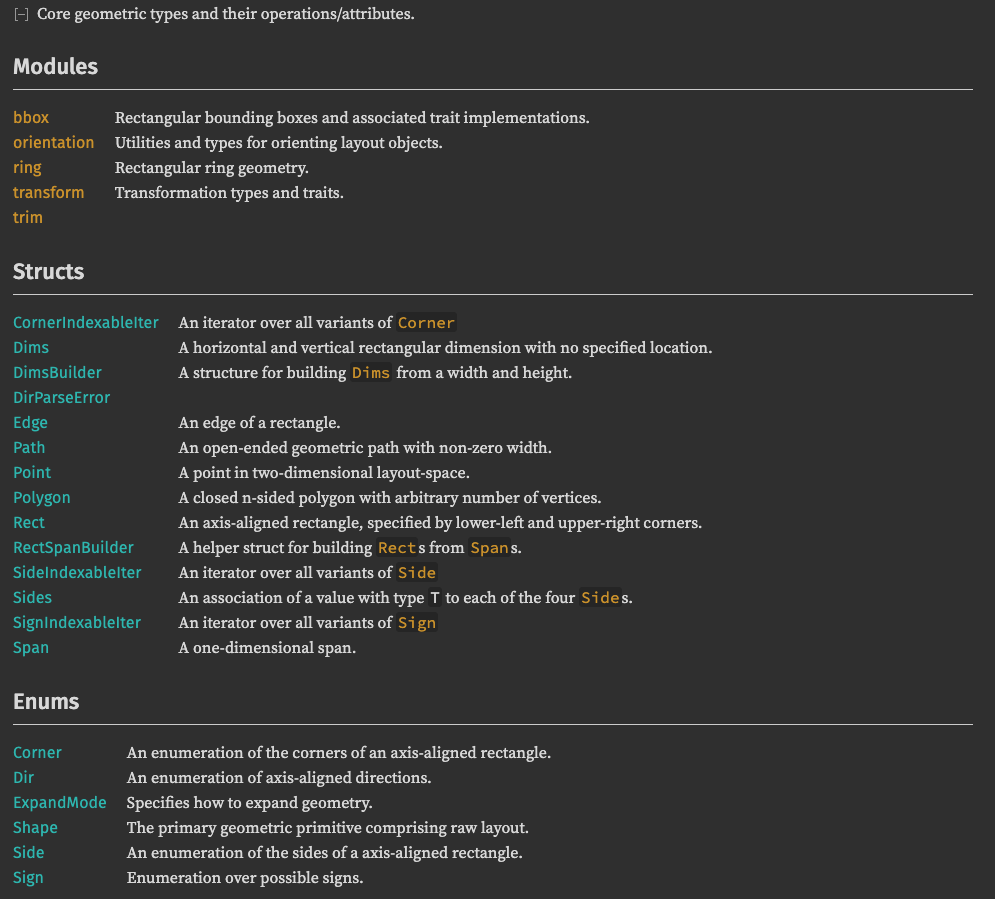
\includegraphics[width=0.8\textwidth]{figures/subgeom.png}
\caption{
    An example page taken from Substrate's geometry API documentation.
}
\end{figure}


The raw layout system provides utilities for:
\begin{itemize}
\item Creating and resizing rectangles.
\item Grouping layout elements (such as rectangles and instances of subcomponents).
\item Relative placement/alignment of layout elements.
\item Rotating/mirroring layout elements and groups of layout elements.
\item Calculating bounding boxes.
\item Flattening hierarchical layout elements.
\item Trimming geometry that lies outside a masking shape.
\end{itemize}

\subsubsection{PDK-provided Unit Cells}

\subsection{Placement Utilities} \label{sec:placement-utilities}

The basis for all placement utilities in Substrate is the \verb|AlignRect| trait,
which provides functions for rectangular/Manhattan positioning for types
that are translatable and have a bounding box.

Users of the \verb|AlignRect| trait specify an \verb|AlignMode|, a reference bounding box or rectangle,
and a spacing. The implementation of the \verb|AlignRect| trait then performs the computations to place
a new bounding box at the requested position relative to the reference box.

The \verb|AlignMode| trait is shown below.

\begin{minted}{rust}
pub enum AlignMode {
    Left,
    Right,
    Bottom,
    Top,
    CenterHorizontal,
    CenterVertical,
    ToTheRight,
    ToTheLeft,
    Beneath,
    Above,
}
\end{minted}

These options generally do what you expect. For example, \verb|AlignMode::Right| aligns the right edges of two boxes,
whereas \verb|AlignMode::ToTheRight| aligns one box to the right of another box.
If a spacing is specified, \verb|AlignMode::ToTheRight| aligns the second box to the right of the first box,
while leaving the desired spacing in between.

Although the alignment API can be directly useful,
it is often more convenient to use higher-level abstractions
when describing the layout of regular (eg. gridded) structures.
To this end, Substrate provides a variety of tiling APIs.

Each of Substrate's tiling implementations takes as input one or more tiles,
as well as metadata about how to place those tiles:
\begin{itemize}
\item The \verb|ArrayTiler| takes a list of tiles, and places them in a vertical or horizontal line.
\item The \verb|GridTiler| takes a 2D array of tiles, and places them in a grid.
\item The nine patch tiler \verb|NpTiler| takes 9 tiles, and two numbers, $n_x$ and $n_y$.
  It tiles these 9 tiles in a manner similar to nine patch images.
  The center tile is repeated in an $n_x \times n_y$ grid.
  The top and bottom edge tiles are repeated in an $n_x \times 1$ array
  directly above and below the center tile grid, respectively.
  The left and right edge tiles are similarly placed in an $n_y \times 1$ array.
  The corner tiles are placed, unrepeated, at the corners of the center tile grid.
\end{itemize}

Each of these tilers uses the raw alignment API to position tiles.
To avoid silent errors, the tiling implementations check that tiles have compatible sizes.
For example, in a grid tiling instance, all tiles in the same column must have the same width,
and all tile in the same row must have the same height.

To ensure that the tiling APIs are composable, the tilers have few requirements
on what can constitute a tile: anything can be tiled, as long as it can be drawn
into a Substrate layout, and it has a bounding box.

This flexibility makes it easy to add new tile types – to mark a type as tileable,
it just needs to be marked with the \verb|CustomTile| trait (which in turn requires
the type to be drawable and have a bounding box). Indeed, Substrate uses
this flexibility internally to provide custom tile types of its own.

For example, it is common to tile objects according to their bounding box
on a specific layer (rather than their overall bounding box).
Tiling standard cells is a common example in which this problem arises.
In Substrate, supporting layer-specific bounding box tiling requires no changes
to the tiler implementation at all.
Instead, Substrate provides the \verb|LayerBbox| tile type, which implements the
aforementioned \verb|CustomTile| trait. The \verb|LayerBbox| constructor takes an inner tile
(eg. a standard cell layout) and a layer identifier, and exposes a standard tile API to the tiler:
\begin{itemize}
\item Drawing a \verb|LayerBbox| tile simply results in drawing the inner tile.
\item When calculating the bounding box, \verb|LayerBbox| filters the elements of the inner tile, considering
  only the elements on its selected layer.
\end{itemize}

Similarly, there is a \verb|Pad| tile type, which adds padding to an inner tile as follows:
\begin{itemize}
\item Drawing the \verb|Pad| tile simply draws the inner tile.
\item The bounding box of the \verb|Pad| tile is the bounding box of the inner tile, expanded by the width of the padding.
\end{itemize}

These custom types are easily composable. For example, you can create a \verb|Pad| tile that wraps a \verb|LayerBbox| tile
that in turn wraps a "regular" tile.


\subsection{Routing} \label{sec:routing}

There are three levels of routing abstraction in Substrate:
1. The lowest level of abstraction deals with routing tracks. This layer provides utilities for calculating
   track locations, locating tracks near a point, and creating half tracks
   (tracks that are half the width of a normal track, with the expectation that two half tracks will abut
   to form a full-size track).
2. The second level of abstraction handles manual routing. This layer is intended for situations in which
   routing performance is important and the rough shape of the route is known in advance. One such situation is
   routing the output of a standard cell inverter to the input of an adjacent inverter. This layer
   provides methods for creating elbow jogs, S-shaped jogs, and collections of multiple parallel jogs.
3. The third and highest level of abstraction is fully automatic gridded routing. Users define a routing grid,
   then request that the router draw routes. Each routing request contains a source location and layer,
   a destination location and layer, and a net name string. Reusing a net name across multiple routing requests
   enables the router to reuse routes previously drawn on that net. The algorithm currently used for routing
   is essentially breadth-first search; the router does not attempt to find globally optimal routes.

Further examples of the routing APIs are given later in this thesis, in the context of SRAM22.


\chapter{SRAM Generator} \label{sec:sram22}

SRAM22 is an open-source SRAM generator for the Skywater 130nm open-source process.
SRAM22 programatically generates SRAM blocks by consuming:
\begin{enumerate}
\item A TOML configuration file, such as the one shown below.
\item A set of hard macros, including standard cells, a sense amplifier, and SRAM bitcells.
\item A summary of process design rules.
\item A Substrate PDK, which provides a parametric transistor generator.
\end{enumerate}

SRAM22 does not attempt to be process-portable, even though many of the above components
can, in principle, be swapped out to port SRAM22 to a new process.

An example TOML configuration file is shown below:

\begin{minted}{toml}
num_words = 32
data_width = 32
mux_ratio = 2
write_size = 32
control = "ReplicaV1"
pex_level = "rcc"
\end{minted}

These options configure the width/depth of the SRAM, the column muxing ratio, and the write mask granularity.
Since running PEX can often take hours or even days, the \verb|pex_level| option allows users to specify
the level of accuracy desired.

An invocation of SRAM22 produces all collateral required for integrating SRAM into a digital flow, including:
\begin{itemize}
\item A SPICE netlist.
\item A GDS layout.
\item A LEF file, identifying pin and blockage locations.
\item A Liberty file, specifying timing constraints.
\item A Verilog behavioral model.
\end{itemize}

Users can also request that SRAM22 run checks on the generated SRAM block, including:
\begin{itemize}
\item Running LVS.
\item Running DRC.
\item Running a sanity-check transistor-level functional simulation.
\end{itemize}

The complete source code for SRAM22 is available on \href{https://github.com/rahulk29/sram22}{GitHub}.
Section \ref{sec:sram-architecture} describes the architecture of the generated SRAM blocks.
Section \ref{sec:sram-layout-generation} describes how SRAM22 programatically generates layout.

\section{Architecture} \label{sec:sram-architecture}

SRAM22 generates self-timed SRAMs. Figure \ref{fig:sram22-block-diagram} shows a block diagram
of the macros generated by SRAM22.

\begin{figure}[H] \centering
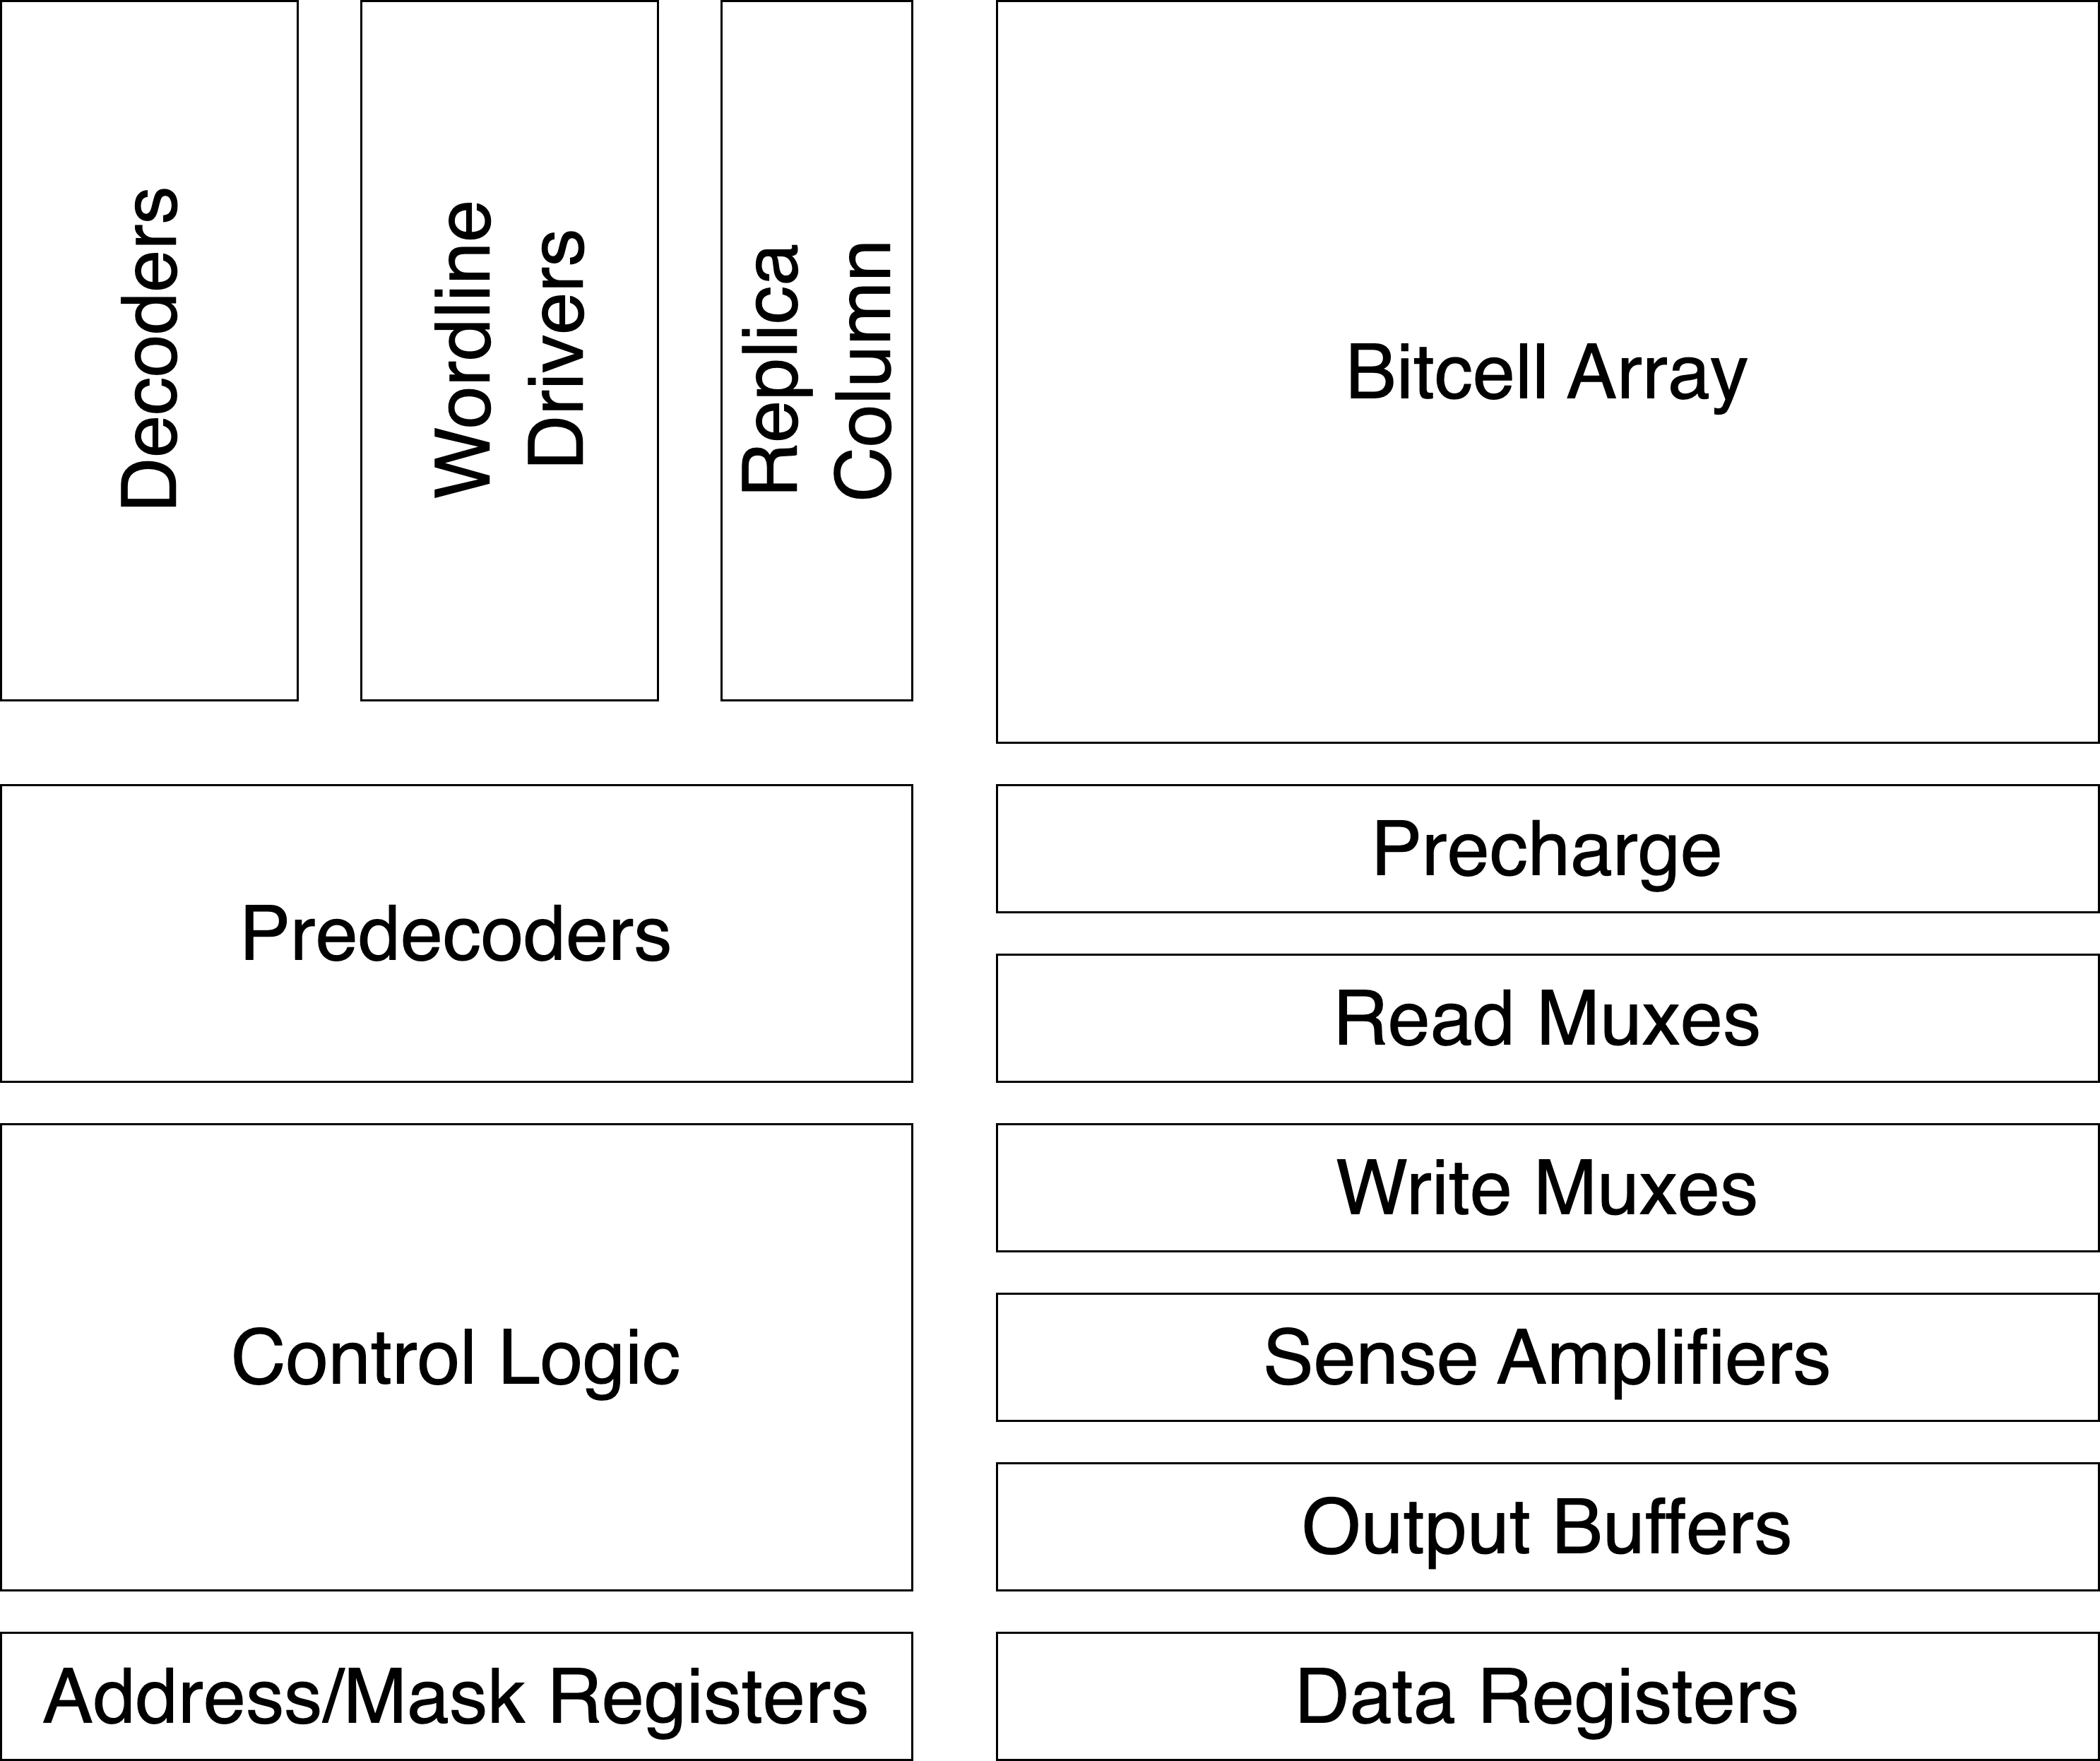
\includegraphics[width=0.8\textwidth]{figures/sram22_block_diagram.png}
\caption{A block diagram of an SRAM macro generated by SRAM22. \label{fig:sram22-block-diagram}}
\end{figure}

The read muxes and write muxes are implemented using PMOS and NMOS pass transistors, respectively.
The sense amplifiers are StrongARM latches. The output buffers ensure symmetric loading of the sense amplifiers.
Figure \ref{fig:col-schematic} shows a schematic of the column circuitry.

\begin{figure}[H]
\begin{center}
\begin{circuitikz}[node distance = 12mm and 20mm]
\usetikzlibrary{calc}
\draw (0,0) node(M1)[pmos, anchor=S, xscale=-1]{}
(M1.D) to[short] ++ (0,-1) node(BL)[circ,label=135:$bl$]{} to[short] ++ (1,0) node(M2)[pmos,anchor=D, rotate=-90]{}
(M2.S) to[short] ++ (1,0) node(BR)[circ, label=45:$\overline{bl}$]{} to[short] ++ (0,1) node(M3)[pmos,anchor=D]{}
(M1.G) -- (M3.G)
(M2.G) to[short] (M2.G |- M1.G) node[circ,midway]{} to[short] ++ (0,1) node[ocirc, label=$\overline{pc}$]{}
(M1.S) node[tground, label=above:$V_{DD}$]{}
(M3.S) node[tground, label=above:$V_{DD}$]{}
(M1.D) to[short] ++ (0,-2) node(MRMUXL)[pmos, anchor=S, xscale=-1]{}
(M3.D) to[short] ++ (0,-2) node(MRMUXR)[pmos, anchor=S]{}
(MRMUXL.D) ++ (0,-2) coordinate(TMP)
;
\draw ($(BL)!0.5!(BR)$) coordinate(TMP2)
(TMP2 |- TMP) node(comp)[fd op amp, rotate=-90]{}
(MRMUXL.D) -| (comp.+)
(MRMUXR.D) -| (comp.-)
(comp.out +) to[short] ++ (0,-0.2) node(bufr)[buffer,anchor=in, rotate=-90, scale=0.5]{}
(comp.out -) to[short] ++ (0,-0.2) node(bufl)[buffer,anchor=in, rotate=-90, scale=0.5]{}
(bufl.out) to[short] ++ (-3,0) to[short] ++ (0, -5) node[ocirc, label=below:$d_{out,n}$]{}
(bufr.out) to[short] ++ (3,0) to[short] ++ (0, -5) node[ocirc, label=below:$d_{out,p}$]{}
(BL) to[short] ++ (-0.5,0) to[short] ++ (0,-2)
to[short] ++ (0,-4.5) node(MLD)[nmos,anchor=D,xscale=-1]{}
(MLD.S) node(MLSEL)[nmos,anchor=D,xscale=-1]{}
(MLSEL.S) node(MLWE)[nmos,anchor=D,xscale=-1]{}
(MLWE.S) node[ground]{}
(BR) to[short] ++ (0.5,0) to[short] ++ (0,-2)
to[short] ++ (0,-4.5) node(MRD)[nmos,anchor=D]{}
(MRD.S) node(MRSEL)[nmos,anchor=D]{}
(MRSEL.S) node(MRWE)[nmos,anchor=D]{}
(MRWE.S) node[ground]{}
;
\draw (0.5,-17) node(DFF)[flipflop D]{}
(DFF.pin 6) |- (MLD.G)
(DFF.pin 4) to[short] ++ (0.5,0) |- (MRD.G)
(MRSEL.G) -- (MLSEL.G) to[short] ++ (-4,0) node[ocirc, label=left:$sel$]{}
(MRWE.G) -- (MLWE.G) to[short] ++ (-4,0) node[ocirc, label=left:$we$]{}
(MRMUXR.G) -- (MRMUXL.G) to[short] ++ (-2, 0) node[ocirc, label=left:$\overline{sel}$]{}
(DFF.pin 1) to[short] ++ (-0.5,0) node[ocirc, label=left:$d_{in}$]{}
(DFF.pin 3) to[short] ++ (-0.5,0) node[ocirc, label=left:$clk$]{}
;
\end{circuitikz}
\end{center}
\caption{SRAM column circuitry. \label{fig:col-schematic}}
\end{figure}

The control logic is a set of digital logic gates that sequences events during each read or write operation.
It contains a pulse generator that detects the rising edge of the clock. These pulses then enable the wordlines
and the replica column. The replica column's bitlines discharge until they cross the threshold
of an inverter, at which point the wordline pulse is disabled and precharge circuitry is activated
to prepare for subsequent operations.
The internally generated sense amplifier clock is also derived
from the replica bitline. Details on the design of the replica timing mechanism can be found in \ref{sec:replica-bitline}.

\subsection{Replica Bitline} \label{sec:replica-bitline}

The purpose of the replica bitline is to accurately track the discharge delay of the true bitlines across
process, voltage, and temperature variations. Since SRAM cells are composed of special transistors
not ordinarily used in logic cells, timing mechanisms based on logic (such as inverter chains) do not
track the true bitlines well.

To minimize power consumption due to charging and discharging the bitlines,
the replica delay can be designed to fire the sense amplifiers when just enough voltage difference
has accumulated. This minimum voltage depends primarily on the sensitivity and offset voltage of the
sense amplifiers.

We present a replica bitline design based on \cite{replicabl}.
We use a design in which there are $N$ replica columns, each of which is smaller than a regular column by a factor of $K$. In other words, if a regular SRAM column has $h$ cells, each replica column will have $h/K$ cells.
The $N$ replica columns are connected in parallel to reduce timing variation due to random effects in active replica cells.
An inverter senses the discharging replica bitline and fires sense amplifiers.
A simplified schematic of the replica circuitry is shown in \ref{fig:replica-schematic}

\begin{figure}[H] \centering
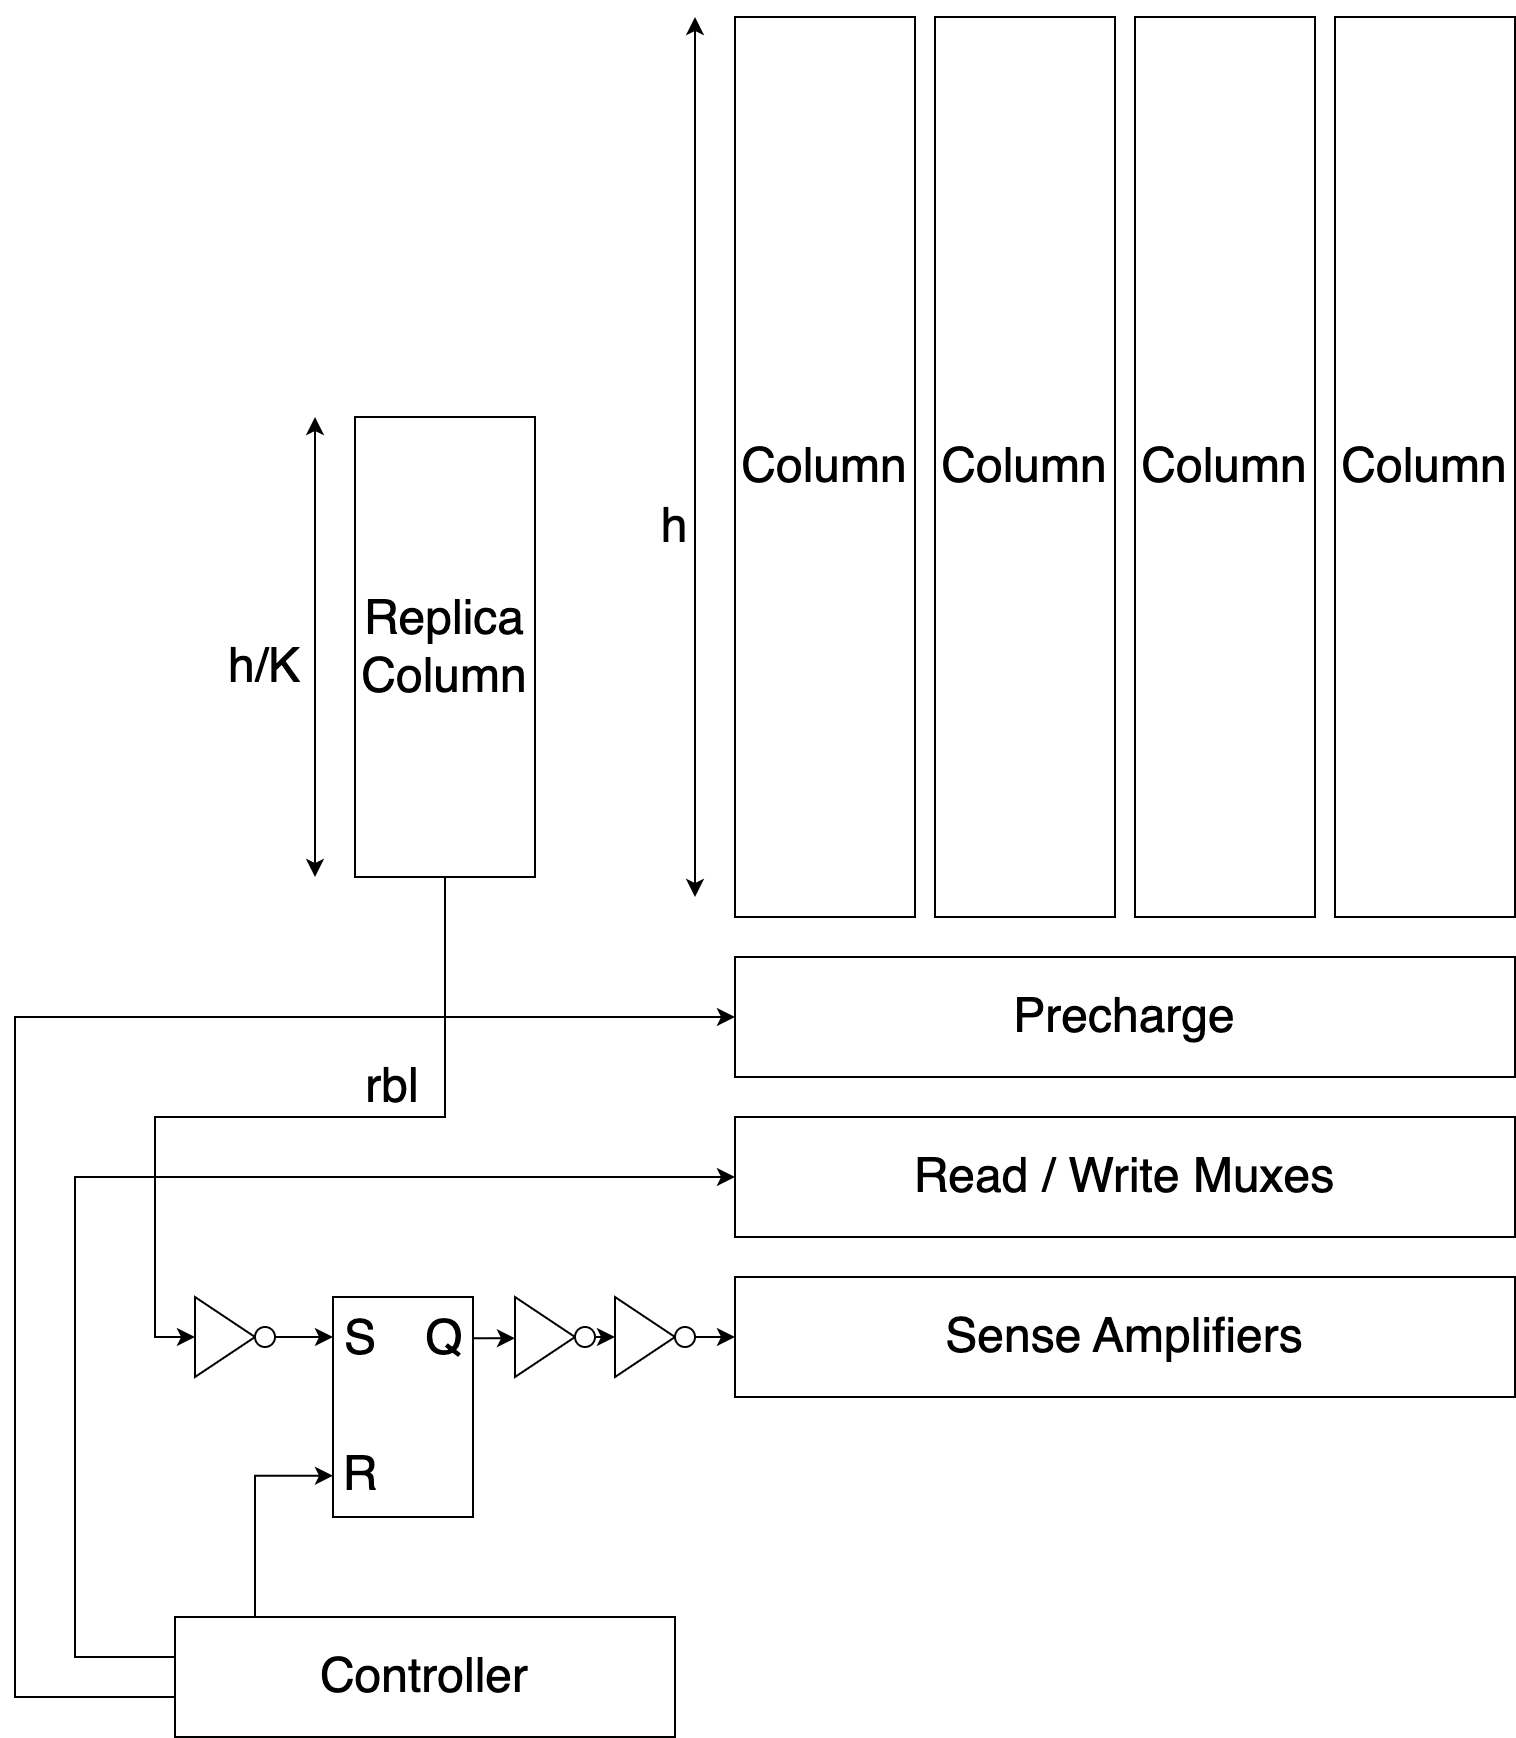
\includegraphics[width=0.8\textwidth]{figures/replica_schematic.png}
\caption{A slightly simplified schematic of the replica circuitry. \label{fig:replica-schematic}}
\end{figure}

We now present a method for selecting the values of $N$ and $K$.

We assume that the following values are known (eg. extracted from simulation) and constant:
\begin{itemize}
\item The bitline capacitance $C_{bl}$
\item The nominal SRAM cell on current, $I_{cell,0}$
\item The standard deviation of SRAM cell current, $\sigma_{I_{cell}}$
\item The standard deviation of the sense amplifier offset voltage $V_{os}$
\item The threshold $V_{flip}$ at which an inverter output flips from low to high
\item The supply voltage $V_{DD}$
\end{itemize}

A read error occurs if the sense amps fire before sufficient voltage difference develops on the true bitlines.

For this analysis, we suppose that we must tolerate up to $M_1$ standard deviations of sense amp offset voltage
and $M_2$ standard deviations of SRAM cell current.

The total bitline capacitance of the replica columns is $ C_{replica} = N/K C_{bl}. $
If this capacitance is discharged by a current $I_{replica}$, the time at which the sense amps are enabled is
\begin{equation}
T_{SAE} = \frac{C_{replica}}{I_{replica}}\left( V_{DD} - V_{flip} \right).
\end{equation}
Note that nominally $I_{replica} = N I_{cell}$, since the replica column contains $N$ replica cells in parallel.

For a correct read, the voltage difference at the input of the sense amps must be larger than $M_1 V_{os}.$
If the true bitlines are discharged by a current $I_{cell}$, we must have
\begin{equation}
T_{SAE} > \frac{C_{bl}}{I_{cell}} M_1 V_{os}.
\end{equation}

The worst case conditions occur when:
\begin{enumerate}
\item The cell being read is slow: $ I_{cell} = I_{cell,0} - M_2 \sigma_{I_{cell}}. $

\item The replica cells are fast: $ I_{replica} = N I_{cell} + M_2 \sqrt{N} \sigma_{I_{cell}}. $

\item The sense amplifiers have the maximal offset voltage $M_1 V_{os}$.
\end{enumerate}

We now derive a condition for correctness under the worst case conditions.

The worst case (earliest) time at which the sense amps are fired is

\begin{equation} \label{eq:tsae-max}
T_{SAE} = \frac{C_{replica}}{I_{replica}} \left( V_{DD} - V_{flip} \right)
= \frac{ N C_{bl}  \left(V_{DD} - V_{flip} \right) }{ K \left( N I_{cell,0} + M_2 \sqrt{N} \sigma_{I_{cell}} \right)}.
\end{equation}

The worst case (latest) time at which sufficient bitline voltage margin has accumulated is

\begin{equation} \label{eq:tmin}
T_{min} = \frac{M_1 C_{bl} V_{os}}{I_{cell} - M_2 \sigma_{I_{cell}}}.
\end{equation}

For correct operation, \ref{eq:tsae-max} must be larger than \ref{eq:tmin}. Thus, the correctness constraint is

\begin{equation} \label{eq:sae-correctness}
\frac{C_{bl}  \left( V_{DD} - V_{flip}\right)}{K \left( I_{cell,0} + M_2 \frac{1}{\sqrt{N}} \sigma_{I_{cell}} \right)} >
\frac{M_1 C_{bl} V_{os}}{I_{cell} - M_2 \sigma_{I_{cell}}}.
\end{equation}

\ref{eq:sae-correctness} shows that increasing $N$ mitigates the variance of the replica cells,
though it does nothing to alleviate the variance of the SRAM cells.

A simple heuristic to select $N$ and $K$ is to solve for $K$ based on the nominal cell current and worst case
sense amp offset voltage:

\begin{align} \label{eq:k-heuristic}
\frac{C_{bl} \left( V_{DD} - V_{flip} \right) }{K I_{cell,0}}
&= \frac{C_{bl} M_1 V_{os}}{I_{cell,0}} \\
\implies K &= \frac{V_{DD} - V_{flip}}{M V_{os}}
\end{align}

The value of $N$ is then determined by finding the minimumm value of $N$ that satisfies \ref{eq:sae-correctness}.
Since $N$ does nothing for the SRAM cell current variation, this approach may not always yield a positive solution for $N$.
Such cases can be solved iteratively by decreasing $K$ and then searching for an $N$ satisfying \ref{eq:sae-correctness}.

Other replica techniques are possible. For example, \cite{niki} uses a larger number of replica bitcells,
resulting in an early sense amp enable signal. This signal is then time-amplified with respect to a clock edge
to generate the final sense amp enable. This excess number of bitcells reduces variation in the sense amp timing
due to replica cell mismatch, but, as with \cite{replicabl}, variation in cell current is not suppressed.
The time amplifier also incurs an area overhead.


\section{Layout Generation} \label{sec:sram-layout-generation}

SRAM22 exercises many of the layout APIs described in \ref{sec:layout-entry}.
This section describes a few representative examples.

This section is organized as follows:
\begin{enumerate}
\item \nameref{sec:bitcell-array-layout} describes how Substrate tiling APIs are used to produce SRAM bitcell arrays from foundry-provided cells.
\item \nameref{sec:precharge-layout} describes how Substrate's raw layout APIs can be used to produce very compact layouts.
\item \nameref{sec:control-logic-layout} describes how Substrate's routing APIs handle custom digital logic, where layout area is dominated
  by standard cell area, rather than by routing performance, and productivity is important.
\end{enumerate}


\subsection{Bitcell Array} \label{sec:bitcell-array-layout}

SRAM22 uses many of the tiling APIs described in \ref{sec:placement-utilities}.
As an example, consider the (toy) 8x8 bitcell array shown in \ref{fig:bitcell8x8}.

\begin{figure}[H] \centering
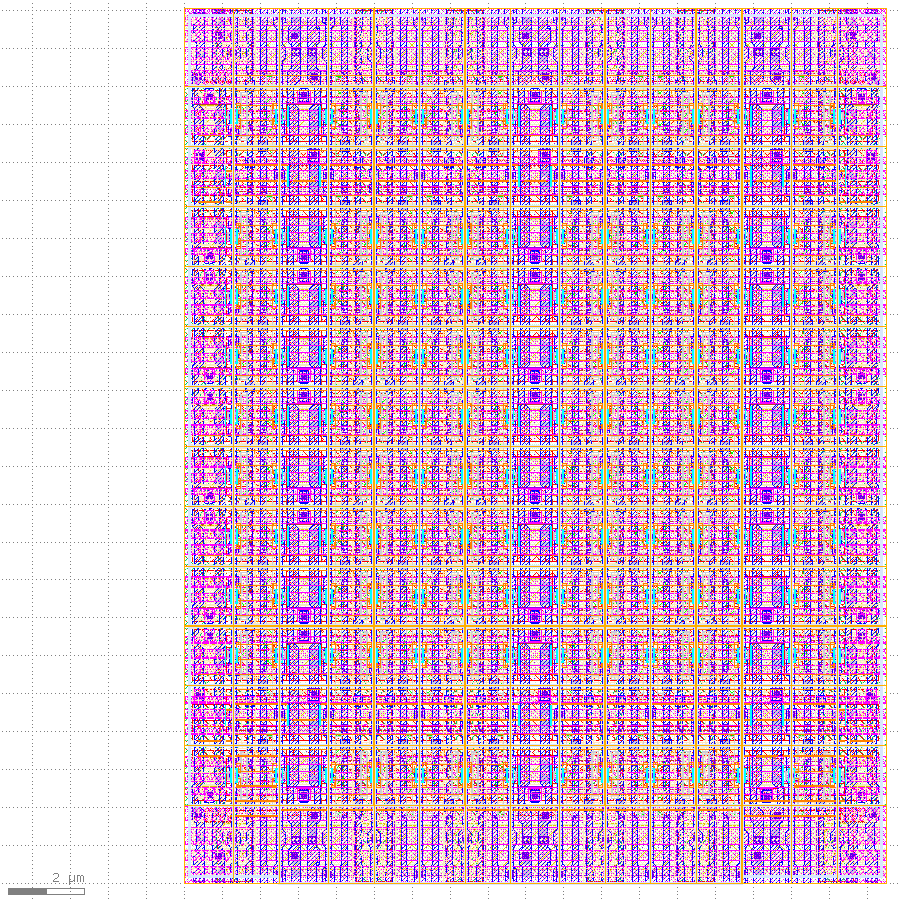
\includegraphics[width=0.8\textwidth]{figures/bitcell8x8.png}
\caption{An 8x8 SRAM bitcell array tiled using Substrate. \label{fig:bitcell8x8}}
\end{figure}

The bitcell array has several structural features commonly found in SRAM bitcell arrays:
\begin{itemize}
\item One horizontal tap row for every 8 rows of cells.
\item One vertical tap column for every 4 columns of cells. Note that this array was
  generated for a column mux ratio of 4. For a column mux ratio of 8, the tap columns
  would be placed every 8 cells.
\item Special row end, column end, and corner cells.
\item Each SRAM bitcell shares bitline and power contacts with its neighbors.
  As a result, each cell in a row is reflected horizontally with respect to the cell preceeding it.
  Similarly, each cell in a column is reflected vertically with respect to the cell above it.
\end{itemize}

The requirements for special edge and corner cells makes this a natural fit for a ninepatch tiler.
To use the ninepatch tiling API, we must first partition the bitcell into the nine ninepatch regions (center, four edges, and four corners).

The center cell is the unit that tiles in both the horizontal and vertical dimensions. For the example shown above,
the center cell contains a horizontal tap row, 8 rows of 4 bitcells, and a vertical tap column. Tiling this cell
will produce an array with the desired frequency of taps (one horizontal tap every 8 rows, and one vertical tap every 4 columns).
An image of the center cell is shown in \ref{fig:bitcell-center}. Note that we have placed taps at the top and left edges of the cell.
We account for this when designing the edge and corner cells.

\begin{figure}[H] \centering
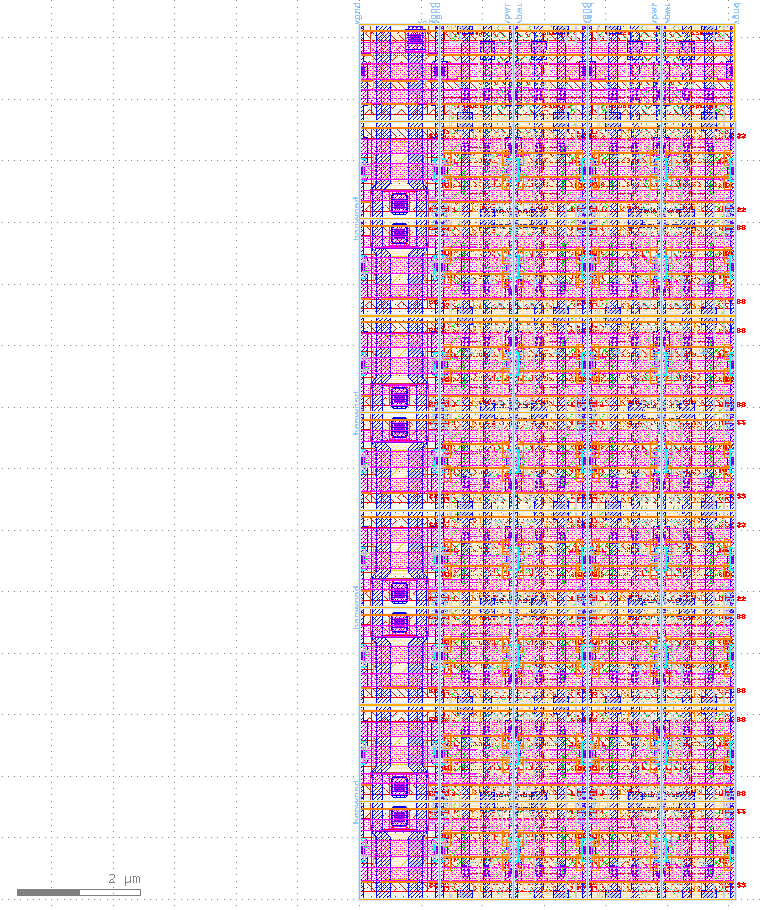
\includegraphics[width=0.5\textwidth]{figures/bitcell_center.png}
\caption{The center ninepatch cell for the bitcell array shown in \ref{fig:bitcell8x8}. \label{fig:bitcell-center}}
\end{figure}

The remainder of the ninepatch tiles are shown in \ref{fig:bitcell-ninepatch-edge-tiles}
and \ref{fig:bitcell-ninepatch-corner-tiles}.

Since the center cell contains taps at the left and top edges, the left/top ninepatch cells
do not contain internal tap structures, whereas the right/bottom cells do.
\begin{figure}[H] \centering
\begin{subfigure}[b]{0.22\textwidth} \centering
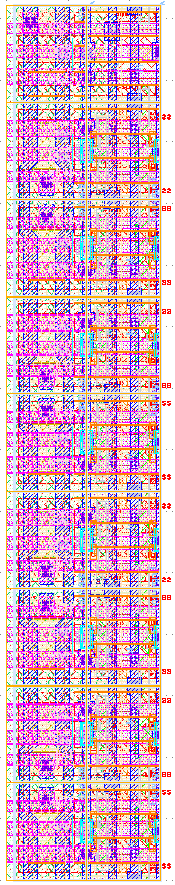
\includegraphics[width=0.7\textwidth]{figures/bitcell_left.png}
\caption{Left edge}
\end{subfigure}
\hfill
\begin{subfigure}[b]{0.22\textwidth} \centering
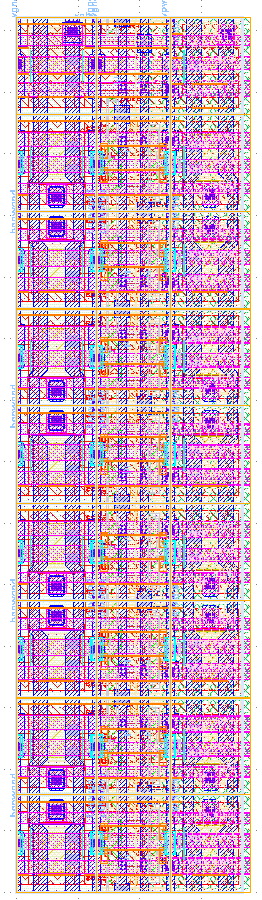
\includegraphics[width=\textwidth]{figures/bitcell_right.png}
\caption{Right edge}
\end{subfigure}
\hfill
\begin{subfigure}[b]{0.22\textwidth} \centering
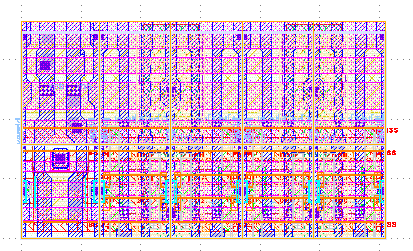
\includegraphics[width=\textwidth]{figures/bitcell_top.png}
\caption{Top edge}
\end{subfigure}
\hfill
\begin{subfigure}[b]{0.22\textwidth} \centering
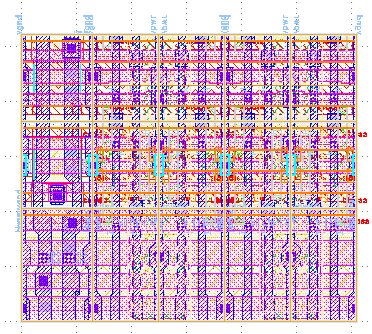
\includegraphics[width=\textwidth]{figures/bitcell_bot.png}
\caption{Bottom edge}
\end{subfigure}

\caption{The four edge ninepatch cells for an SRAM bitcell array. \label{fig:bitcell-ninepatch-edge-tiles}}
\end{figure}

\begin{figure}[H] \centering
\begin{subfigure}[b]{0.22\textwidth} \centering
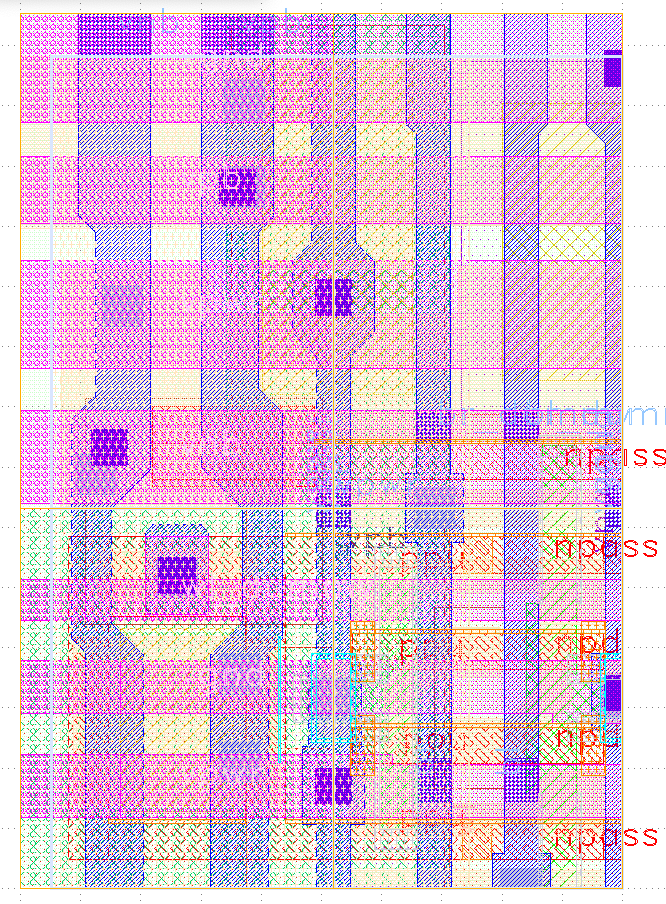
\includegraphics[width=\textwidth]{figures/bitcell_ul.png}
\caption{Upper left}
\end{subfigure}
\hfill
\begin{subfigure}[b]{0.22\textwidth} \centering
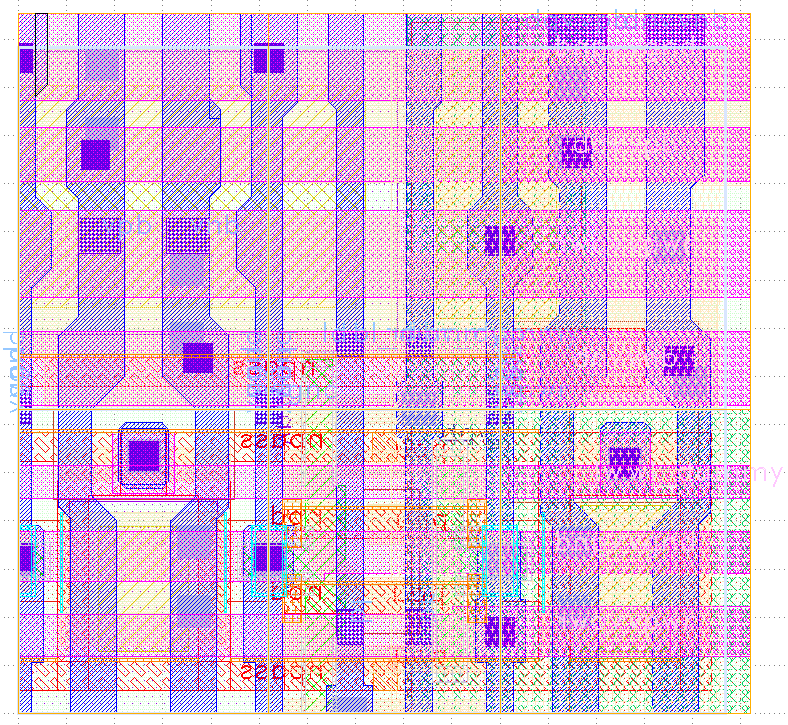
\includegraphics[width=\textwidth]{figures/bitcell_ur.png}
\caption{Upper right}
\end{subfigure}
\hfill
\begin{subfigure}[b]{0.22\textwidth} \centering
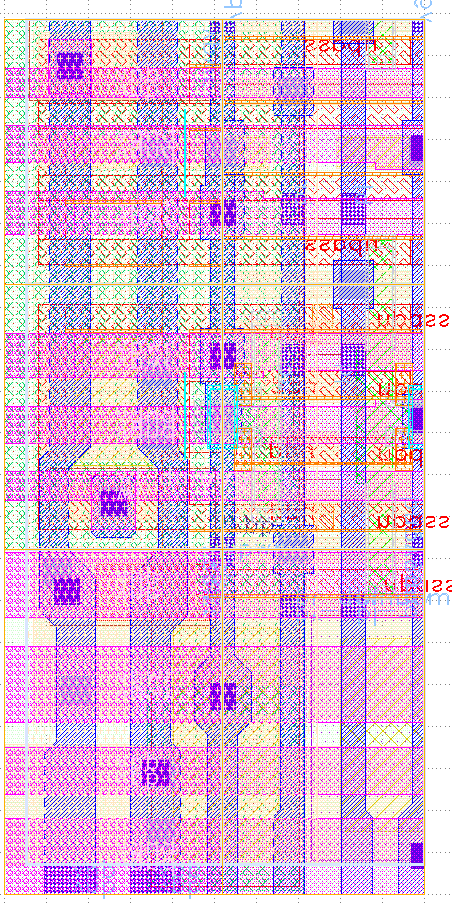
\includegraphics[width=\textwidth]{figures/bitcell_ll.png}
\caption{Lower left}
\end{subfigure}
\hfill
\begin{subfigure}[b]{0.22\textwidth} \centering
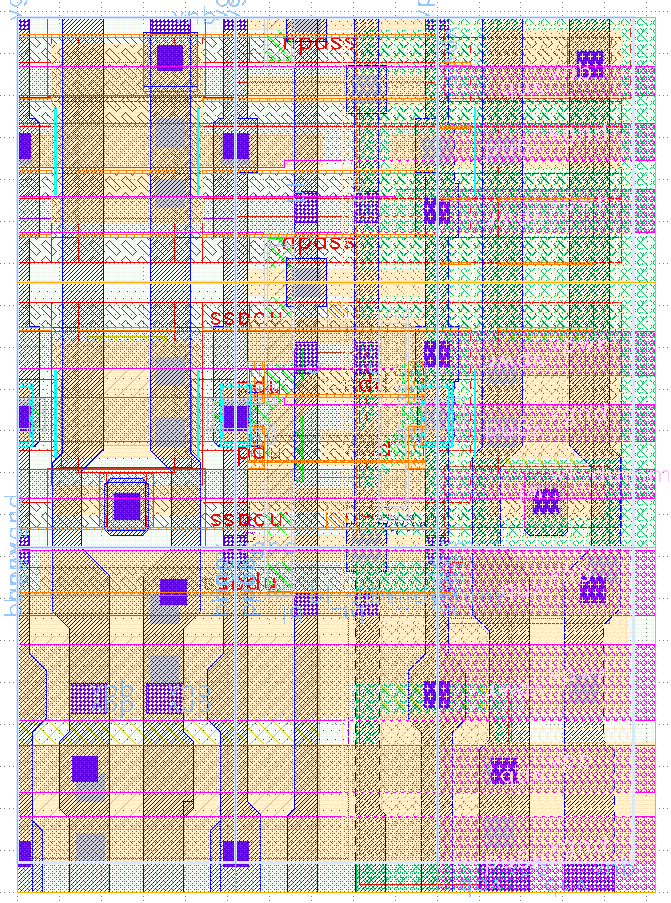
\includegraphics[width=\textwidth]{figures/bitcell_lr.png}
\caption{Lower right}
\end{subfigure}

\caption{The four corner ninepatch cells for an SRAM bitcell array. \label{fig:bitcell-ninepatch-corner-tiles}}
\end{figure}

% #figure(
%   table(
%     columns: 4,
%     align: center,
%     image("figures/bitcell_left.png", width: 22%),
%     image("figures/bitcell_right.png", width: 22%),
%     image("figures/bitcell_top.png", width: 22%),
%     image("figures/bitcell_bot.png", width: 22%),
%     image("figures/bitcell_ul.png", width: 22%),
%     image("figures/bitcell_ll.png", width: 22%),
%     image("figures/bitcell_ur.png", width: 22%),
%     image("figures/bitcell_lr.png", width: 22%),
%   ),
%   caption: [
%     The off-center ninepatch cells for the bitcell array shown in @bitcell8x8.
%     Top row (from left to right): left edge, right edge, top edge, bottom edge.
%     Bottom row (from left to right): upper left corner, lower left corner, upper right corner, lower right corner.
%   ],
% ) <bitcell-ninepatch-tiles>

Once we have generated layouts of the ninepatch cells, tiling them 
using Substrate's \verb|NpTiler| is fairly straightforward:

\begin{minted}{rust}
// Build a ninepatch tiler using 9 patch cells.
let tiler = NpTiler::builder()
    .set(Region::CornerUl, &corner_ul)
    .set(Region::Left, &left)
    .set(Region::CornerLl, &corner_ll)
    .set(Region::Top, &top)
    .set(Region::Center, &center)
    .set(Region::Bottom, &bot)
    .set(Region::CornerUr, &corner_ur)
    .set(Region::Right, &right)
    .set(Region::CornerLr, &corner_lr)
    .nx(nx)
    .ny(ny)
    .build();
\end{minted}

Each of the nine ninepatch region tiles are composite cells; they each contain
multiple foundry-provided primitive cells. To generate these tiles, we use Substrate's \verb|GridTiler|.

For example, \ref{fig:bitcell-left-cell-code} shows a portion of the code for generating the left edge cell.
\begin{figure}[H] \centering
\begin{minted}{rust} 
// Create a row of SRAM tiles.
let cell_row: Vec<OptionTile> = into_vec![rowend_replica, cell];
// Create a row of SRAM + OPC tiles.
let cell_opt1a_row: Vec<OptionTile> = into_vec![rowenda_replica, cell_opt1a];
// Create a row of tap tiles.
let hstrap: Vec<OptionTile> = into_vec![rowend_hstrap, hstrap];

// Build a grid from the rows created above.
let mut grid = Grid::new(0, 0);
grid.push_row(hstrap);
for _ in 0..self.params.hstrap_ratio / 2 {
    grid.push_row(cell_opt1a_row.clone());
    grid.push_row(cell_row.clone());
}

// Tell Substrate to place the cells according
// to their positions in the grid.
let mut grid_tiler = GridTiler::new(grid);
\end{minted}
\caption{A code snippet for generating the left edge cell of an SRAM bitcell array. \label{fig:bitcell-left-cell-code}}
\end{figure}

This code:
\begin{enumerate}
\item Creates three rows of 2 cells each: one normal bitcell row, one bitcell row with slight modifications
  to geometry for OPC, and one row for taps. These rows are just collections of cells; they are not
  yet placed in the actual cell layout.
\item Adds the tap row as the first (topmost) row in the grid. This row will align with the topmost row
  of the ninepatch center cell (\ref{fig:bitcell-center}), which is also a tap row.
\item Adds alternating rows of regular bitcells and modified-OPC bitcells. Eight rows are added in total,
  since \verb|self.params.hstrap_ratio| is 8 here. As is evident from the code, the frequency of horizontal
  tap rows can easily be adjusted.
\item Creates a \verb|GridTiler| instance to place all of the cells.
\end{enumerate}

The lowest level of cells in the hierarchy (eg. \verb|cell|, \verb|cell_opt1a| in the code above) are imported
into Substrate using hard macros (\ref{sec:hard-macros}).

In addition to tiling geometry, we also expose relevant ports from each of the tilers. This allows
other generators to figure out how to connect to the bitcell array. For example, we expose ports for
each of the wordlines, bitlines, and power strap connections. The code to do this is omitted for brevity,
but can be found in the SRAM22 source code.

Although bitcell tiling is not fundamentally a hard problem, we believe that the approach of decomposing
the problem into reasonably intuitive parts (such as grid and ninepatch tiling) is better and more easily understood
than the alternative, ``simpler'' method of writing a double for loop
with edge cases to handle the array edge cells and periodic taps.

\subsection{Precharge} \label{sec:precharge-layout}

The precharge cell illustrates how to use Substrate to produce compact, tileable layouts.
The SRAM bitcell width in the Skywater 130nm process is \SI{1.2}{\micro\meter}.
The minimum metal 1 line and space is \SI{0.28}{\micro\meter},
meaning that at most 4 M1 tracks will fit within the bitcell pitch. However, since minimum-sized vias are wider
than the minimum M1 width, we are practically limited to around 3 M1 tracks. There are four signals involved
in the precharge circuit: the bitline, complementary bitline, VDD, and active low precharge enable.
Thus, routing performance is critical.
The precharge cell is very simple: it contains two pull-up transistors and an equalizing transistor.
The schematic is shown in \ref{fig:precharge-schematic}.

% \draw (0,0) node[tground, label=above:$V_{DD}$]{}
% to[american current source, l=$I_b$] ++ (0,-2)
% node(M2)[nmos, anchor=D, label=right:$M_2$]{}
% (M2.S) node(M1)[nmos, anchor=D, label=right:$M_1$]{}
% (M1.S) node[ground]{}
% (M1.G) node[ocirc,label=left:$V_{in}$]{}
% (M1.D) to[short] ++ (1.5,0) to[C=$C_P$] ++ (0,-1.5) node[ground]{}
% (M2.G) node[ocirc, label=left:$V_{bias}$]{}
% (M2.D) to[short] ++ (2.5,0) coordinate(TMP)
% to[C=$C_L$] ++ (0,-1.5) node[ground]{}
% (TMP) to[short] ++ (2,0) coordinate(TMP)
% to[R=$R_L$] ++ (0,-1.5) node[ground]{}
% (TMP) to[short]++ (1,0) node[ocirc,label=right:$V_{out}$]{}

\begin{figure}[H]
\begin{center}
\begin{circuitikz}[node distance = 12mm and 20mm]
\draw (0,0) node(M1)[pmos, anchor=S, xscale=-1]{}
(M1.D) to[short] ++ (0,-1) node[circ]{} to[short] ++ (1,0) node(M2)[pmos,anchor=D, rotate=-90]{}
(M2.S) to[short] ++ (1,0) node[circ]{} to[short] ++ (0,1) node(M3)[pmos,anchor=D]{}
(M1.G) -- (M3.G)
(M2.G) to[short] (M2.G |- M1.G) node[circ,midway]{} to[short] ++ (0,1) node[ocirc, label=$\overline{pc}$]{}
(M1.S) node[tground, label=above:$V_{DD}$]{}
(M3.S) node[tground, label=above:$V_{DD}$]{}
(M1.D) to[short] ++ (0,-3) node[ocirc, label=below:$BL$]{}
(M3.D) to[short] ++ (0,-3) node[ocirc, label=below:$\overline{BL}$]{}
;
\end{circuitikz}
\end{center}
\caption{Precharge cell schematic. \label{fig:precharge-schematic}}
\end{figure}

The final precharge cell layout is shown in \ref{fig:precharge-final}.

\begin{figure}[H] \centering
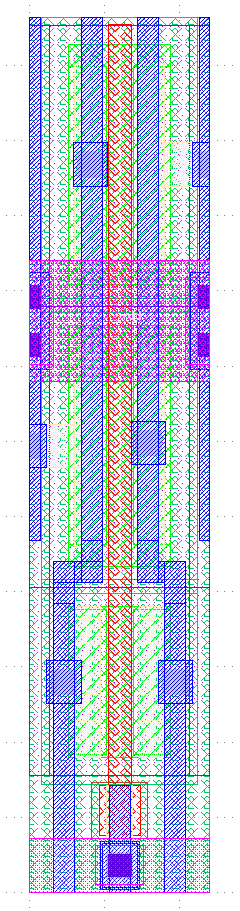
\includegraphics[angle=90, width=\textwidth]{figures/precharge_final.png}
\caption{The pitch-matched precharge cell in SRAM22. \label{fig:precharge-final}}
\end{figure}

Before we describe how SRAM22 generates this layout, we first highlight some important features:
\begin{itemize}
\item VDD is routed into the cell from metal 2 (pink) and drops onto split tracks on metal 1 (blue).
  The split tracks of adjacent cells abut to form a full track.
\item The bitlines jog slightly to make space to enable routing precharge enable to the gates of the precharge devices.
\item The total capacitance (and therefore total wire length) on the bitline and bitline complement nets must be approximately equal.
\end{itemize}

To generate the precharge cell layout, we start by instantiating the three precharge transistors, as shown in \ref{fig:precharge-transistors}.

\begin{figure}[H] \centering
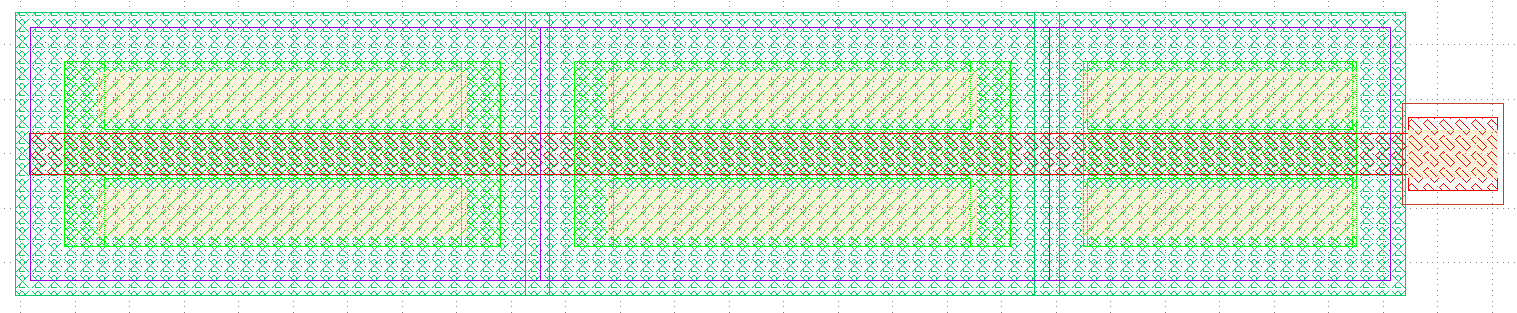
\includegraphics[width=0.75\textwidth]{figures/precharge_transistors.png}
\caption{The three base transistors of a precharge cell. \label{fig:precharge-transistors}}
\end{figure}

\begin{figure}[H] \centering
\begin{minted}{rust}
let params = LayoutMosParams {
  skip_sd_metal: vec![vec![]; 3],
  deep_nwell: true,
  // Place all gate contacts on one side of the transistor stack.
  contact_strategy: GateContactStrategy::SingleSide,
  // Create three FETs with the given dimensions.
  devices: vec![
      MosParams {
          w: self.params.equalizer_width,
          l: self.params.length,
          m: 1,
          nf: 1,
          id: mos.id(),
      },
      MosParams {
          w: self.params.pull_up_width,
          l: self.params.length,
          m: 1,
          nf: 1,
          id: mos.id(),
      },
      MosParams {
          w: self.params.pull_up_width,
          l: self.params.length,
          m: 1,
          nf: 1,
          id: mos.id(),
      },
  ],
};

let mut mos = ctx.instantiate::<LayoutMos>(&params)?;
// Rotate the devices 90 degrees.
mos.set_orientation(Named::R90);
\end{minted}
\caption{A snippet of code for generating the precharge transistors shown in \ref{fig:precharge-transistors}. \label{fig:precharge-transistors-code}}
\end{figure}

Next, we allocate M1 routing tracks. At the left edge of the cell, the outermost half-tracks are used for routing VDD;
the inner two tracks are the bitlines. Towards the right side of the cell,
the bitline tracks move to make space for the gate contact.

These two routing regions are encoded using a \verb|FixedTracks| object in Substrate, connected by a \verb|SimpleJog|.
The \verb|FixedTracks| object produces tracks with a fixed line and space, centered in a given routing region.
It also accepts boundary conditions, which permit the user to place full tracks, half tracks, full spaces, or half spaces
at the edge of the routing region.

The \verb|SimpleJog| object allows the user to specify an arbitrary number of source tracks, and an equal number of destination tracks.
It then jogs each source track to the corresponding destination track.

A code snippet (lightly edited for clarity) and image of this stage of precharge cell generation are shown in \ref{fig:precharge-m1-routing-code} and \ref{fig:precharge-m1-routing}.

\begin{figure}[H] \centering
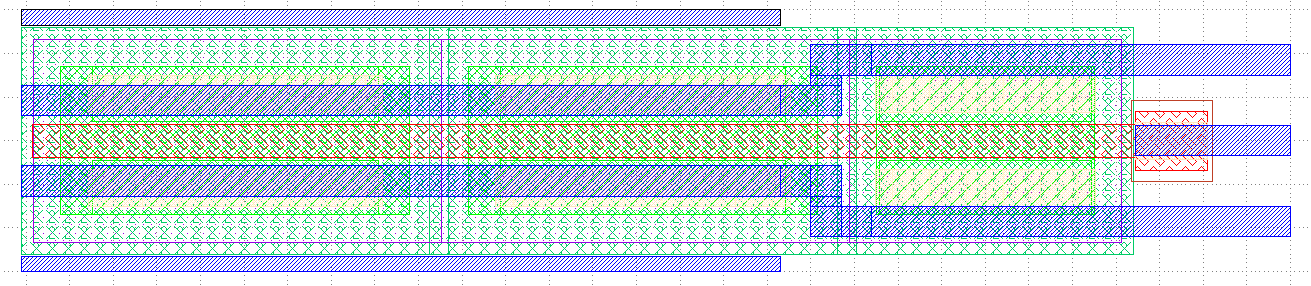
\includegraphics[width=0.75\textwidth]{figures/precharge_m1_routing.png}
\caption{Precharge cell metal 1 routing. \label{fig:precharge-m1-routing}}
\end{figure}

\begin{figure}[H] \centering
\begin{minted}{rust}
// Create two sets of fixed tracks.
let in_tracks = FixedTracks::from_centered_tracks(CenteredTrackParams {
    line: 140,
    space: 230,
    span: Span::new(0, 1_200),
    num: 4,
    lower_boundary: Boundary::HalfTrack,
    upper_boundary: Boundary::HalfTrack,
    grid: 5,
});
let out_tracks = FixedTracks::from_centered_tracks(CenteredTrackParams {
    line: 140,
    space: 230,
    span: Span::new(0, 1_200),
    num: 3,
    lower_boundary: Boundary::HalfSpace,
    upper_boundary: Boundary::HalfSpace,
    grid: 5,
});

// ...

// Jog between the track regions.
let jog = SimpleJog::builder()
    .dir(Dir::Vert)
    .src_pos(cut)
    .src([dsn.out_tracks.index(0), dsn.out_tracks.index(2)])
    .dst([dsn.in_tracks.index(1), dsn.in_tracks.index(2)])
    .line(dsn.v_line)
    .space(dsn.v_space)
    .layer(dsn.v_metal)
    .build()
    .unwrap();

// Extend the tracks beyond the jog up to the bounding box height.
for i in 0..dsn.in_tracks.len() {
    let rect = Rect::from_spans(
        dsn.in_tracks.index(i),
        Span::new(jog.dst_pos(), bbox.height()),
    );
    ctx.draw_rect(dsn.v_metal, rect);
}
\end{minted}
\caption{A snippet of code for generating precharge cell M1 routing.
The resulting layout is shown in \ref{fig:precharge-m1-routing}. \label{fig:precharge-m1-routing-code}}
\end{figure}


Next, we draw vias connecting the metal 1 tracks to transistor sources/drains/gates.
We also draw a power strap on metal 2 and drop vias to the VDD tracks on metal 1.
Sample code for drawing a via is shown in \ref{fig:sample-via-code}.
The \verb|ViaExpansion::LongerDirection| flag shown in that figure tells the via generator
that the via need not be contained in the overlap of the geometry on the top and bottom layers;
it can expand along the longer direction of the overlap region. This produces the 2x1 via arrays
seen in \ref{fig:precharge-vias}. If no expansion is permitted, Substrate fills the overlap region with as many
vias as possible. At least one via will be drawn, even if it does not fit entirely within the overlap region.

The precharge cell after drawing all vias and the power strap is shown in \ref{fig:precharge-vias}.

\begin{figure}[H] \centering
\begin{minted}{rust}
let mut via1 = ViaParams::builder()
  .layers(dsn.v_metal, dsn.h_metal)
  .expand(ViaExpansion::LongerDirection)
  .geometry(rects[0].double(Side::Left), stripe)
  .build();
let via = ctx.instantiate::<Via>(&via1)?;
ctx.draw(via)?;
\end{minted}
\caption{
Sample code snippet for drawing a via.
\label{fig:sample-via-code}
}
\end{figure}

\begin{figure}[H] \centering
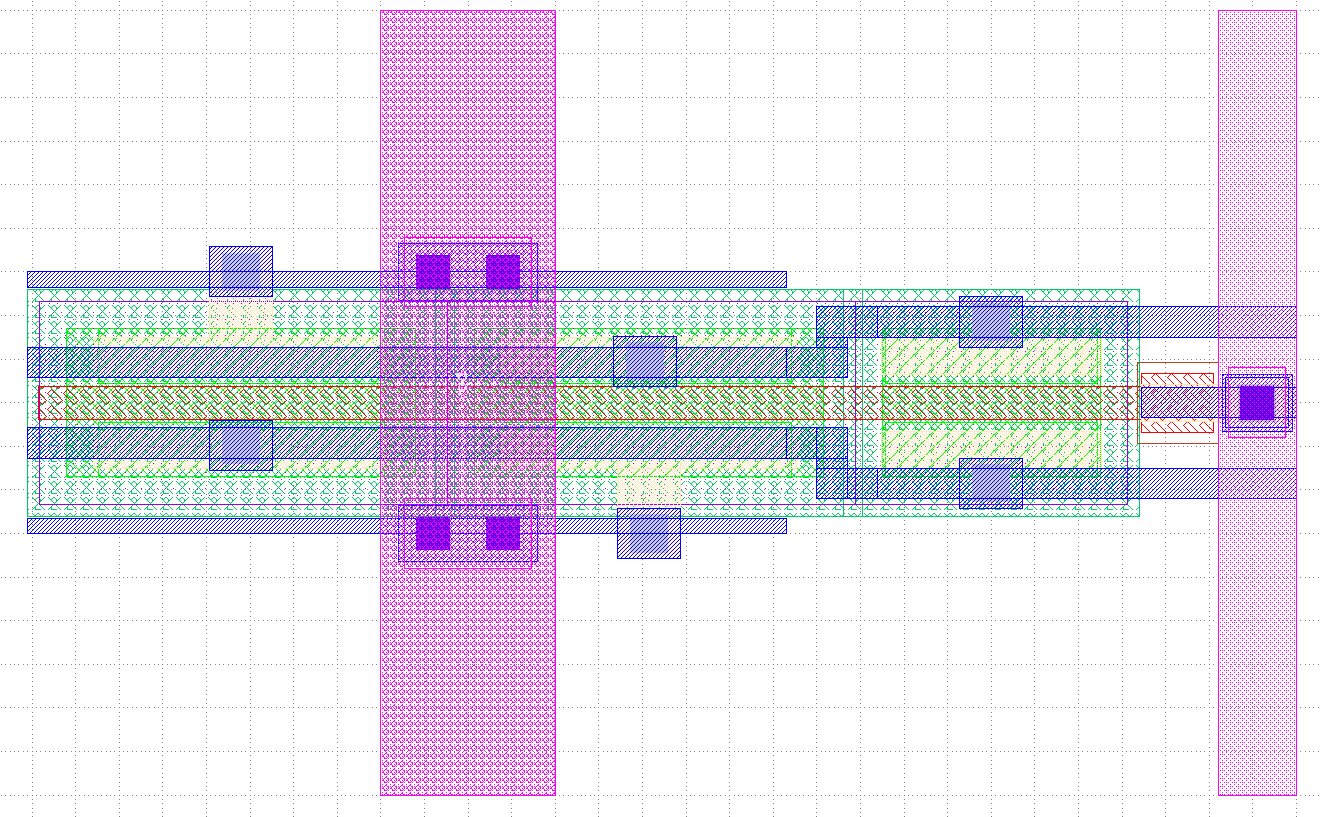
\includegraphics[width=0.75\textwidth]{figures/precharge_vias.png}
\caption{The precharge cell after drawing vias and a power strap. \label{fig:precharge-vias}}
\end{figure}


Finally, as shown in \ref{fig:precharge-trimmed}, we trim the precharge cell so that it can be tiled (using the tiling APIs described previously).

\begin{figure}[H] \centering
\begin{minted}{rust}
let bounds = ctx.brect().with_hspan(Span::new(0, dsn.width));
ctx.trim(&bounds);
\end{minted}
\caption{Trimming the precharge cell. \label{fig:precharge-trimmed}}
\end{figure}

There is an alternate convention for tiling cells, which is to skip the step of trimming the cell, and instead
allow adjacent cells to overlap. However, the convention of trimming cells is more convenient here for two reasons:
\begin{enumerate}
\item Substrate tilers place cells according to their bounding boxes. Tiling untrimmed cells would require wrapping them
  in a \verb|LayerBbox| tile (see \ref{sec:placement-utilities}) or manually specifying the bounding box to the tiler. Trimming the cell is more convenient than
  either of these options.
\item Special end cells are required to provide taps. So even if we were to tile untrimmed cells, we would still need to specify custom cells for
  the array edges and tap columns.
\end{enumerate}

The precharge cells illustrate how Substrate APIs can be used to produce very compact layout.
Much of the SRAM peripheral circuitry is generated in a similar manner. An image of the peripheral circuitry layout
is shown in \ref{fig:peripheral-circuitry-layout}. We omit specific discussion of the generators for the rest of the column
components, since they are similar in principle to the precharge cell.

\begin{figure}[H] \centering
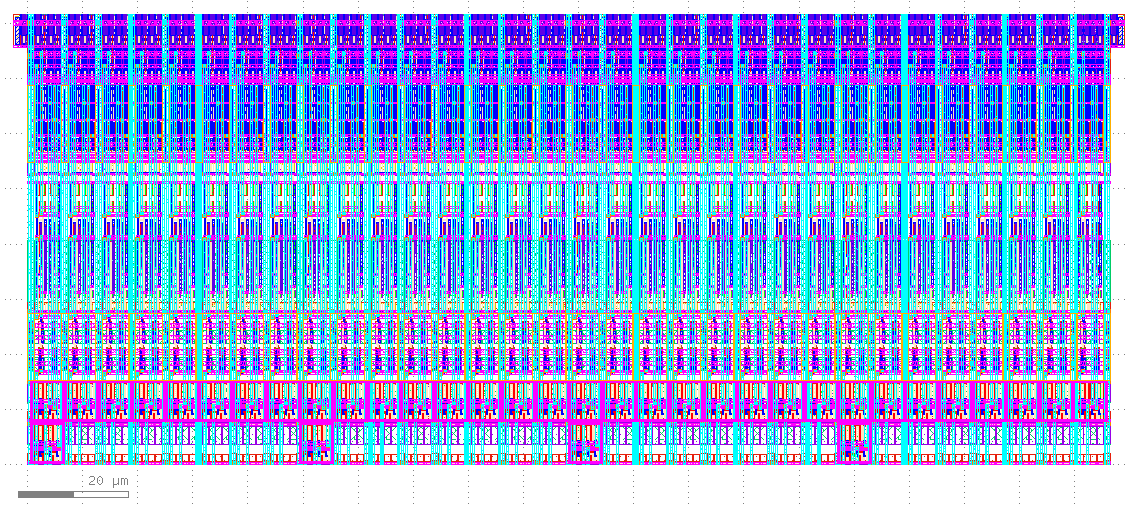
\includegraphics[width=\textwidth]{figures/col_peripherals.png}
\caption{Tiled column peripheral circuitry. The precharge cells occupy the topmost row. \label{fig:peripheral-circuitry-layout}}
\end{figure}

\subsection{Control Logic} \label{sec:control-logic-layout}

The control logic is a small $\left( \approx 100\right)$ set of logic gates that control the sequence of events during read and write operations.

Despite being entirely digital, using a traditional digital flow to lay out the control logic is undesirable:
\begin{itemize}
\item The control logic is pulsed, unlike the typical digital circuits for which these tools are optimized.
\item Minimizing area is important.
\item SRAM22 tries not to depend on commercial tools, and open source digital tool flows are not very mature.
\item Dependency on external tools would make SRAM22 more difficult and less convenient to use.
\end{itemize}

Therefore, we opt instead to place and route the control logic entirely within SRAM22 and Substrate.

The flow for using digital standard cells in Substrate is:
\begin{enumerate}
\item Import the desired standard cell libraries into Substrate.
\item Place the standard cells, often using a \verb|GridTiler| (\ref{sec:placement-utilities}) with tiles taking their bounding box from a ``PR boundary'' layer.
\item Select routing layers and define a routing grid for each layer.
\item Route between the placed standard cells.
\end{enumerate}

The fourth step is often done with a combination of manual routing and automatic routing.
SRAM22 uses manual routing when drawing routes than run solely on the local interconnect layer in SKY130.
For longer distance routes that span other metal layers, SRAM22 defers routing to the automatic router in Substrate.

We will focus on the use of the automatic router in this section, since this feature is, as far as we are aware, not present
in other analog generator frameworks. The router implementation in Substrate is called \verb|GreedyRouter|, as it creates
routes as they are specified, rather than trying to find a globally optimal routing solution.

To initialize the router, we specify a routing region and a set of routing layers. Each routing layer holds the
line and space of tracks on that layer, a preferred routing direction, and a reference to a PDK layer.
Router intialization is shown in \ref{fig:greedy-router-initialization}.

\begin{figure}[H] \centering
\begin{minted}{rust}
let mut router = GreedyRouter::with_config(GreedyRouterConfig {
    area: group.brect().expand(1840),
    // Allow routing on 2 layers: M1 and M2.
    layers: vec![
        LayerConfig {
            line: 320,
            space: 140,
            dir: Dir::Horiz,
            layer: m1,
        },
        LayerConfig {
            line: 320,
            space: 140,
            dir: Dir::Vert,
            layer: m2,
        },
    ],
});
\end{minted}
\caption{Greedy router initialization with two metal layers (M1 and M2). \label{fig:greedy-router-initialization}}
\end{figure}

The current implementation of \verb|GreedyRouter| only permits on-grid routing.
However, cells being routed may have off-grid pins. These pins must be jogged onto
the routing grid before asking the router to route from/to them. Substrate
provides an \verb|expand_to_grid| function for doing this. An example usage is shown in \ref{fig:router-expand-to-grid}.
Users specify a rectangle representing the off-grid pin and an expansion strategy. The router
will automatically find an appropriate on-grid point to which the off-grid pin can be connected,
consistent with the expansion strategy. Possible expansion strategies include:
\begin{itemize}
\item Minimum area: connect to the routing grid using the minimum amount of extra metal area.
\item Top/bottom/left/right: connect to the nearest grid point to the given side of the source pin.
\item Upper left/lower left/upper right/lower right: connect to the nearest grid point off of the given corner of the source pin.
\end{itemize}

\begin{figure}[H] \centering
\begin{minted}{rust}
let clkp_out = router.expand_to_grid(
    clkp_out_via.layer_bbox(m1).into_rect(),
    ExpandToGridStrategy::Minimum,
);
router.occupy(m1, clkp_out, "clkp")?;
\end{minted}
\caption{Expanding the (pulse generator output) pin to the routing grid. \label{fig:router-expand-to-grid}}
\end{figure}


Substrate also has more sophisticated routines for bringing off-grid geometry onto the routing grid.
For example, users can ask the Substrate router to jog a bus of off-grid pins onto adjacent routing tracks.
The router will calculate the minimum necessary amount of spacing in the routing layer's preferred routing direction.
The router logic can handle a wide range of off-grid pitches, and can handle cases where the off-grid bus is not centered
with the target on-grid tracks. An example of the geometry generated by this procedure is shown in \ref{fig:off-grid-routing}.

\begin{figure}[H] \centering
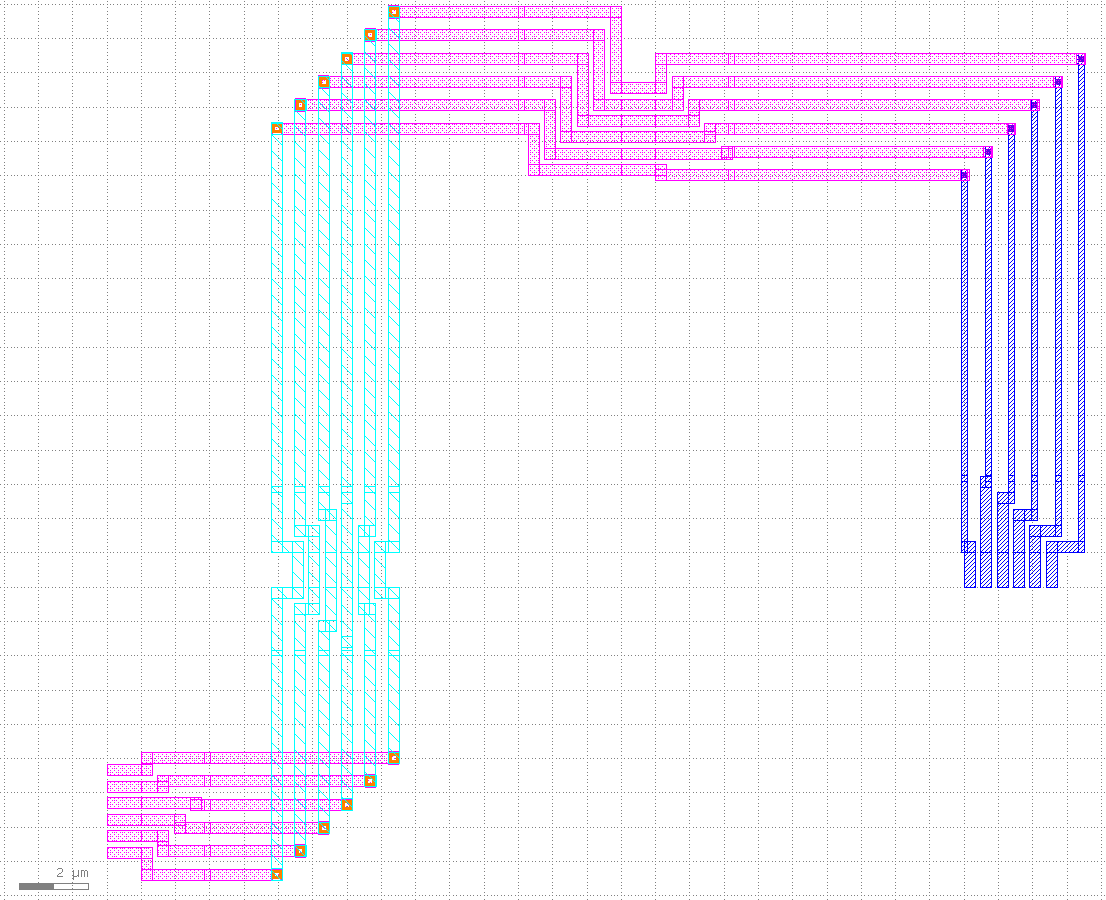
\includegraphics[width=\textwidth]{figures/off_grid_routing.png}
\caption{A sample of the geometry automatically generated by the router to bring off-grid pins to the routing grid. \label{fig:off-grid-routing}}
\end{figure}


Bringing off-grid pins to the routing grid is by far the most tedious part of generating layouts based on
digital standard cells. Further improvements to Substrate have the potential to make this process easier.

Once all geometry is on-grid, routing becomes very easy (see \ref{fig:auto-routing}).

\begin{figure}[H] \centering
\begin{minted}{rust}
router.route_with_net(ctx, m1, clkp_out, m1, clkp_in_1, "clkp")?;
router.route_with_net(ctx, m1, clkp_out, m1, clkp_in_2, "clkp")?;
router.route_with_net(ctx, m1, clkp_out, m1, clkp_in_3, "clkp")?;
\end{minted}
\caption{Routing the clock pulse generator output to three consumers. \label{fig:auto-routing}}
\end{figure}
    % Routing the clock pulse generator output \texttt{(\verb|clkp_out|)} to three consumers \texttt{(\verb|clkp_in_1|, \verb|clkp_in_2|, \verb|clkp_in_3|)}.
    % The net name "clkp" identifies that each route is on a net called "clkp"; this tells the router that it can
    % reuse any geometry previously drawn on the same net. Without this, a naive routing implementation might try to find
    % separate, independent routes from \texttt{\verb|clkp_out|} to each of the three targets.

By issuing several of these routing commands, the full layout can be programatically routed. Extracting these
routing paths from a schematic view is possible in principle, but has not been implemented at the time of writing.

The fully-routed layout of SRAM22's control logic is shown in \ref{fig:control-logic-routed-layout}. The output pins are placed towards
the upper right for convenience in top-level routing.

\begin{figure}[H] \centering
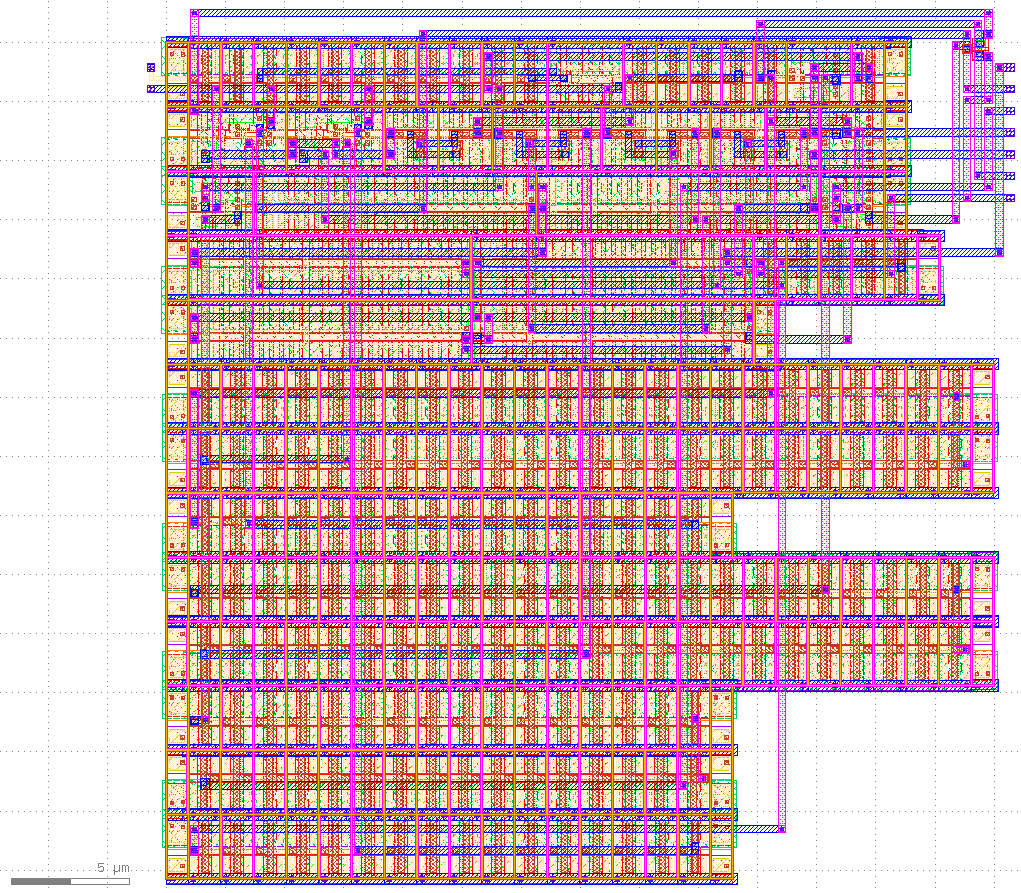
\includegraphics[width=\textwidth]{figures/control_logic_layout.png}
\caption{The control logic cell in SRAM22. Most routing is done via the automatic router in Substrate. \label{fig:control-logic-routed-layout}}
\end{figure}


\chapter{Conclusion} \label{sec:conclusion}

This thesis presented Substrate, a new framework for analog generators
written in the Rust programming language, as well as SRAM22, a configurable
SRAM generator built on top of Substrate.

\section{Additional Features}

Substrate has many features beyond the ones described in this thesis.
In particular, Substrate provides APIs for functional verification
and for verifying digital timing constraints (eg. setup/hold times)
in contexts where analog workflows are more convenient.
The latter feature was used to design and verify a schematic-level tree serializer
generator intended for die-to-die links. Substrate is also capable
of generating power straps compatible with Hammer, the VLSI
flow tool developed at Berkeley \cite{hammer}.

\section{Future Work}

There are a wide variety of directions for future work.
We suggest a few here.

\begin{itemize}
\item Designing an intermediate representation for representing circuits.
Such an intermediate representation would be useful to enable faster
design space exploration, and could enable greater interoperability between generator frameworks.
\item Smarter algorithms for analog routing. In particular, it would be nice to have 
an automatic router capable of generating symmetric/matched differential routing,
while understanding which nets are aggressors and which are victims.
\item Easing the process of integrating analog IP into digital flows, a process
that currently requires setting up flows for several tools not often used in a purely-analog workflow.
Instantiating macros in digital flows is usually done outside of the generator framework,
but there are benefits to having the generator be aware of how it integrates into a digital-top floorplan.
Power strap consistency is one such example.
Utilities for quickly setting up analog/digital co-simulation would also make the process of analog
integration easier.
\end{itemize}


\printbibliography

% \appendix
% \chapter{More Monticello Candidates}

\end{document}

